\documentclass[orivec]{llncs}
\usepackage{graphicx}
\usepackage{amsmath}			% for "cases"
\usepackage{amsfonts}			% for frakur fonts
\usepackage{mathrsfs}			% for curly "E" error symbol
\usepackage{float}
\usepackage[most]{tcolorbox}	% for wrapping example in color box
% \usepackage{wrapfig}		% wrap figure beside text, used in example
\usepackage{tikz-cd}			% commutative diagrams
\usepackage{tikz}
\usepackage{amssymb}			% for \multimap \updownarrow \bigstar \varnothing
\usepackage{sectsty}			% change section color
% \usepackage{turnstile}		% longer turnstiles
\usepackage{wasysym}			% smileys
\usepackage[normalem]{ulem}	% underline with line breaks: /uline
\usepackage{hyperref}			% refs, links become clickable
\usepackage[]{algorithm2e}		% algorithms
%\usepackage[3D]{movie15}	% for embedding 3D shapes
%\usepackage[UKenglish]{babel}	% for movies or 3D
%\usepackage{media9}			% *** doesn't work

\usepackage{geometry}		% change paper size
\geometry{
  a4paper,         % or letterpaper
  textwidth=18cm,  % llncs has 12.2cm
  textheight=27cm, % llncs has 19.3cm
  heightrounded,   % integer number of lines
  hratio=1:1,      % horizontally centered
  vratio=2:3,      % not vertically centered
}
\usepackage[fontsize=13pt]{scrextend}

% *************** Delete when not using Chinese or colors **********************
\usepackage{xeCJK}
\setCJKmainfont[BoldFont=SimHei,ItalicFont=KaiTi]{SimHei}
\usepackage{color}
\definecolor{cerulean}{RGB}{100,100,200}
\definecolor{darkgreen}{RGB}{10,130,10}
%\newcommand{\emp}[1]{\emp{\textcolor{Cerulean}{#1}}}
\newcommand{\emp}[1]{{\color{blue}\textbf{#1}}}
\definecolor{grey}{rgb}{0.98,0.98,0.98}
\definecolor{lightyellow}{rgb}{0.98,0.98,0.90}

% \chapterfont{\color{blue}}		% sets colour of chapters
\sectionfont{\color{blue}} 
\subsectionfont{\color{blue}} 
\subsubsectionfont{\color{blue}} 
\setcounter{secnumdepth}{3}		% use numbers in subsubsections
% \renewcommand\thesection{}		% hide section numbers (has bad indent effect)
% let\emptyset\varnothing			% more beautiful empty set symbol
\newcommand{\vect}[1]{\boldsymbol{#1}}
\newcommand*\sigmoid{\raisebox{-.2\height}{
\includegraphics{sigmoid.png}}}
\newcommand*\stepfunction{\vcenter{\hbox{
\includegraphics{step-function.png}}}}
\newcommand*\KB{\vcenter{\hbox{
\includegraphics{KB-symbol.png}}}}
\newcommand*\NN{\vcenter{\hbox{\includegraphics{NN-symbol.png}}}}
\newcommand*\invsigmoid{\vcenter{\hbox{\includegraphics{inverse-sigmoid.png}}}}
\newcommand{\invW}{\, \rotatebox[origin=c]{90}{W}}
\newcommand{\invw}{\, \rotatebox[origin=c]{90}{w}}
\newcommand*\rectifier{\vcenter{\hbox{\includegraphics{rectifier.png}}}}
\newcommand{\dashh}{\textemdash~}
\newcommand{\tab}{\hspace*{1cm}}

\newcommand{\tikzmark}[1]{\tikz[overlay,remember picture] \node (#1) {};}

\let\labelitemi\labelitemii

\renewcommand{\thefootnote}{\fnsymbol{footnote}}
\interfootnotelinepenalty=10000

% ***** Boxed variables inside math equations
% \newcommand*{\boxedcolor}{black}
\makeatletter
% \renewcommand{\boxed}[1]{\textcolor{\boxedcolor}{%
% \fbox{\normalcolor\m@th$\displaystyle#1$}}}
% \setlength{\fboxsep}{1pt}
\renewcommand{\boxed}[1]{\fbox{\m@th$\displaystyle\scalebox{0.9}{#1}$} \,}
\makeatother

\overfullrule=0mm

\newsavebox{\MyName}
\savebox{\MyName}{
\includegraphics[scale=0.6]{YKY.png}}

\title{什么是神经网络?\\
{\normalsize(中学数学程度可懂)}}
\titlerunning{What are neural networks?}
\author{\usebox{\MyName} (King-Yin Yan)
% \\ \footnotesize{General.Intelligence@Gmail.com}
}
\institute{General.Intelligence@Gmail.com}

\begin{document}

\maketitle
\setlength{\parindent}{0em}
% \setlength{\parskip}{2.8ex plus0.8ex minus0.8ex}
\setlength{\parskip}{2.8ex}

%\begin{abstract}
%\end{abstract}

人工智能中最重要的 3 大技术是:
\begin{itemize}
 \item 逻辑
 \item 神经网络
 \item 进化
\end{itemize}
神经网络属於统计学习 (statistical learning) 的一种,这些方法将 vector space 中的某些「点」分类。

Deep learning 的意思,简单来说,是「\emp{很多层}的神经网络」。 深度学习是目前人工智能中最备受瞩目的一种技巧。

\section*{生物的神经细胞}

温习一下在中学时学过的生物学 {\Large \smiley}

这是一粒真的神经元:
\begin{equation}
\vcenter{\hbox{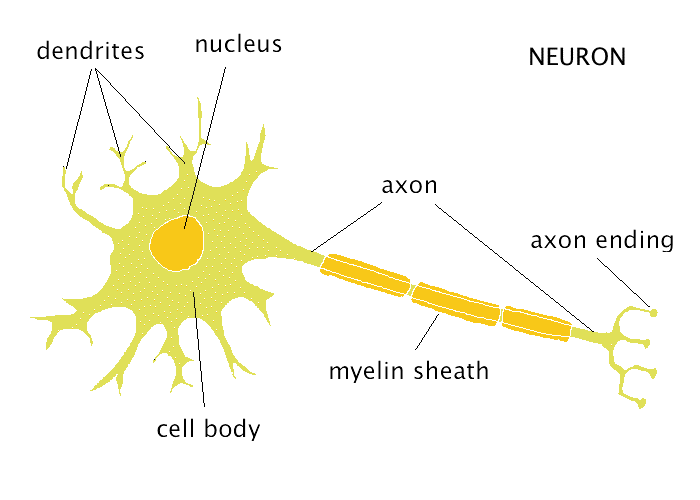
\includegraphics[scale=0.4]{neuron.png}}}
\end{equation}
细胞周围的 dendrites \emp{收集}电信号,当这些脉冲信号的\emp{总和}超过某一阀值 (threshold) 时,会\emp{发射} (fire) 一个电脉冲信号,从 axon 输出到另一神经元:

\begin{equation}
\vcenter{\hbox{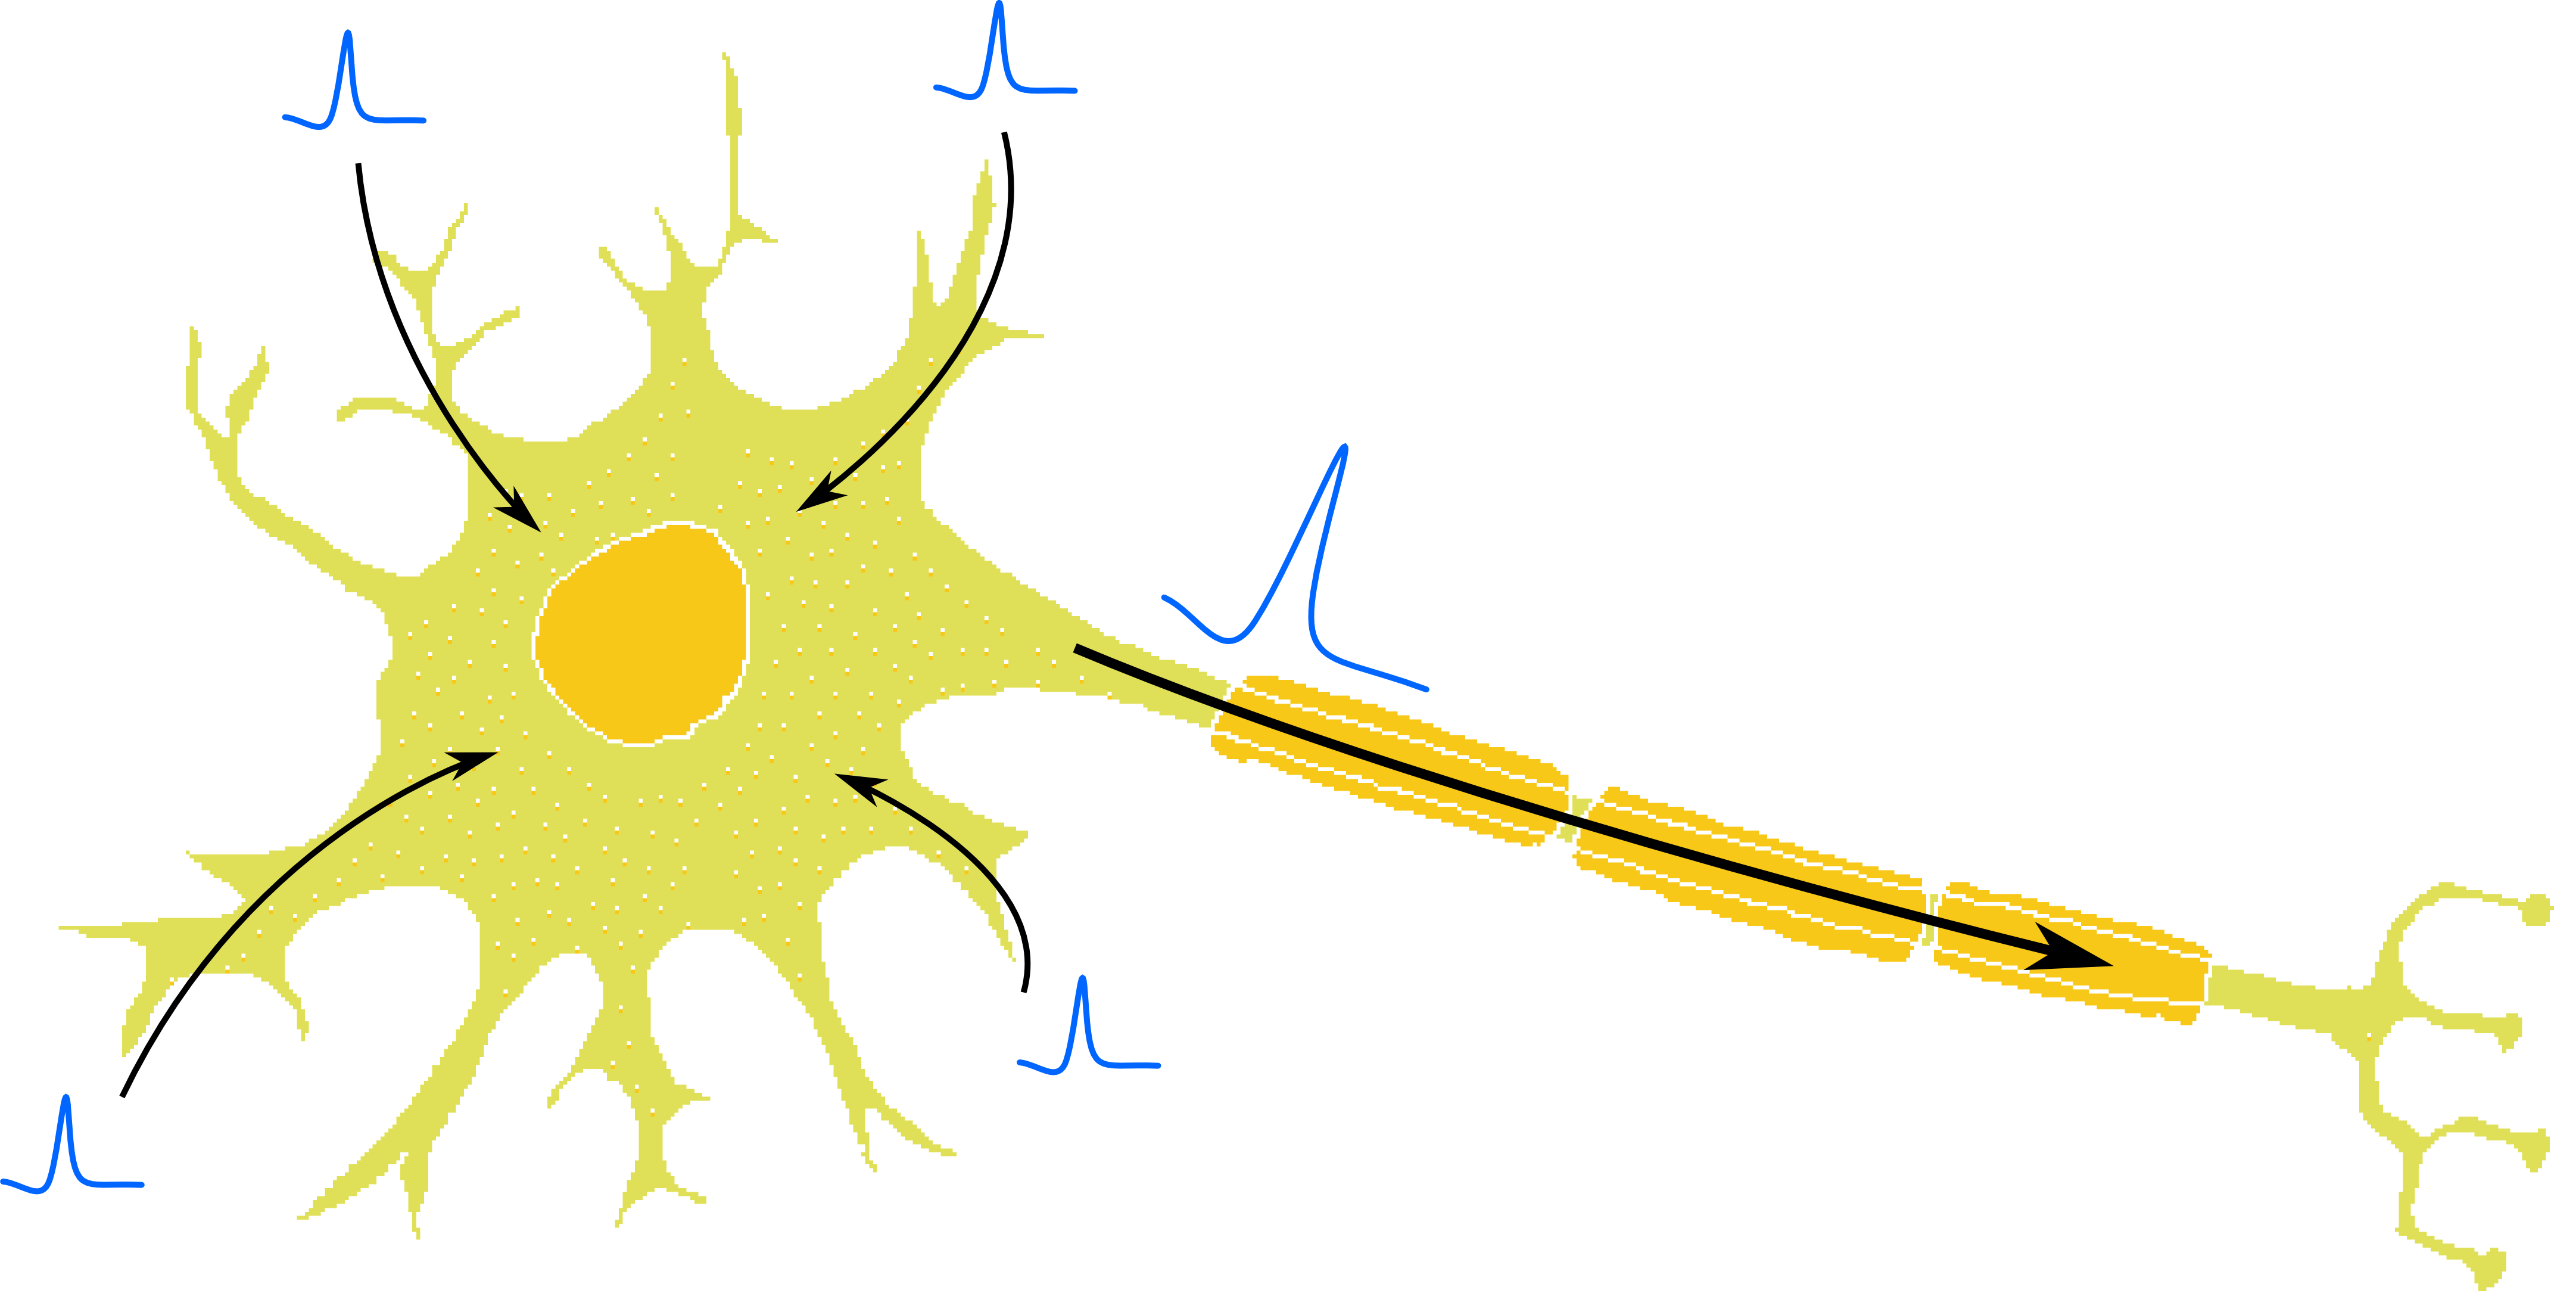
\includegraphics[scale=0.5]{neuron-firing.png}}}
\end{equation}
数学上我们将这过程极度简化,变成这样的模型 (model):
\begin{equation}
\vcenter{\hbox{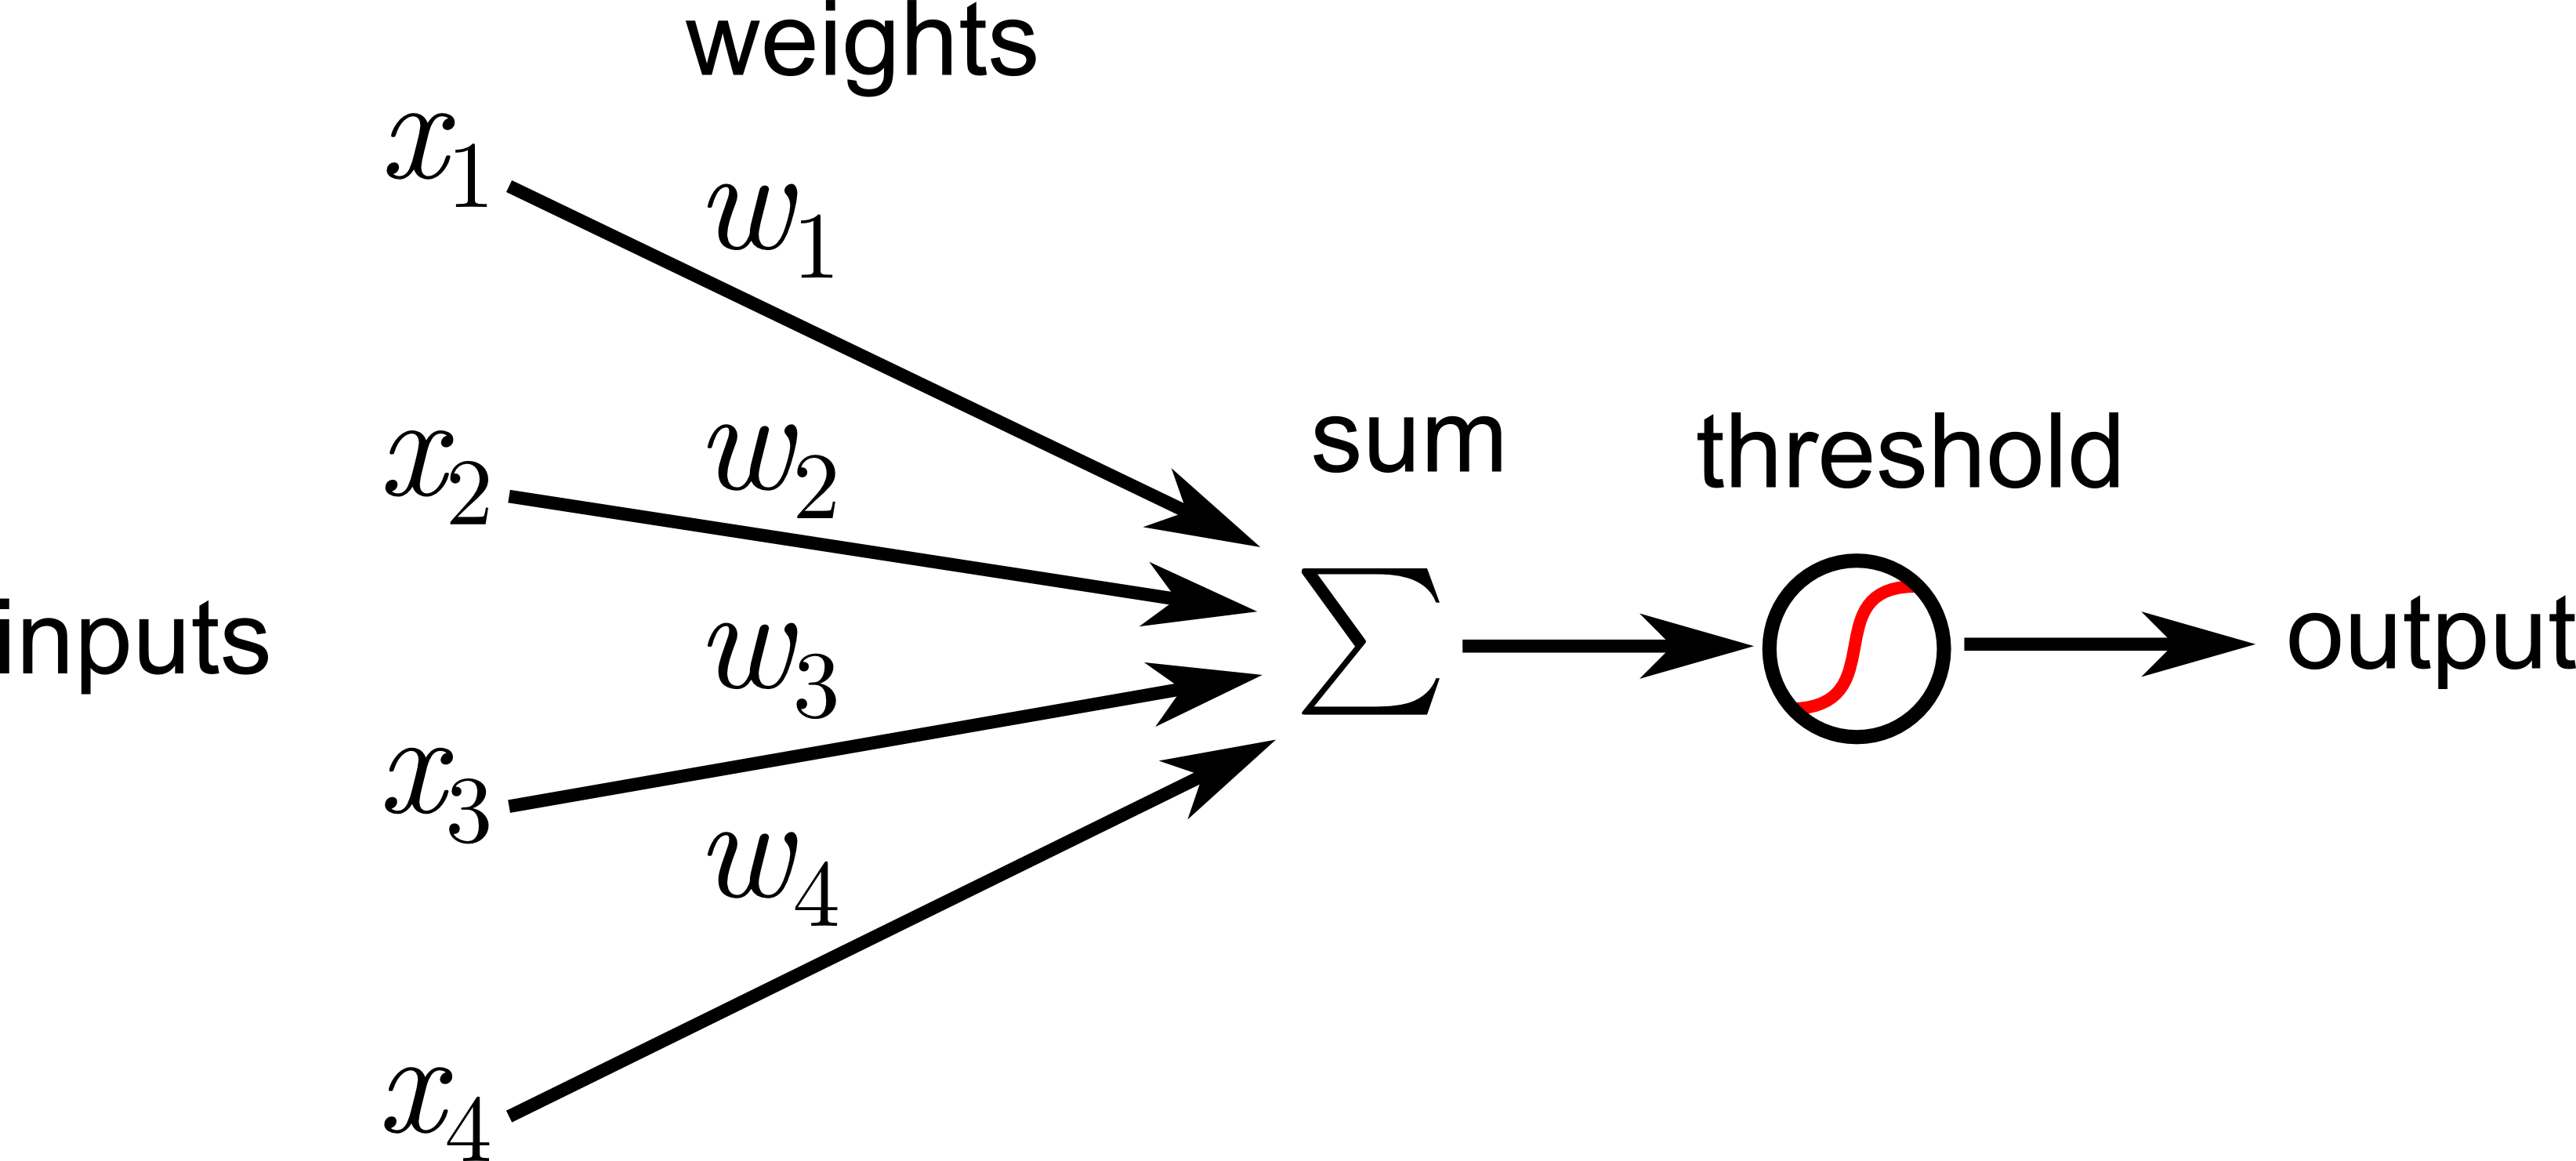
\includegraphics[scale=0.75]{neuron-model.png}}}
\end{equation}
意思是: 将每个输入加权 (weighted) 加起来,然后经过一个 $\sigmoid$ 形状的函数输出。 

用数式表示:
\begin{equation}
\boxed{output} \; y = \sigmoid \; [ \; \sum_i (w_i \; x_i) \; ]
\end{equation}
其中 $\sigmoid$ = sigmoid 函数是:
\begin{equation}
\sigmoid (x) = \frac{1}{1 + e^{-x}}
\end{equation}
它的形状是这样的:
\begin{equation}
\vcenter{\hbox{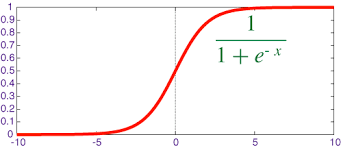
\includegraphics[scale=0.55]{sigmoid-graph.png}}}
\end{equation}
它代表在左边没有信号 (0 = nothing),在右边的信号值是 1 = ``yes''。

其实也可以用以下这些函数模拟 threshold 的作用:
\begin{equation}
\vcenter{\hbox{\includegraphics[scale=0.5]{../AGI-17/activation-functions.png}}}
\end{equation}

\begin{tcolorbox}[colback=lightyellow, breakable, enhanced]
\emp{Fun fact \#1}\\

神经细胞的表面布满了 sodium-potassium (Na$^+$/K$^+$) channels,它们用 ATP (adenosine triphosphate, 细胞的能量来源)以 3 Na$^+$ : 2 K$^+$ 的比例将 ions「泵」到细胞内,造成电压差。 这些蓄势待发的电压,当电压超过 threshold 时某些 channels 打开,造成 ``action potential''。 这个现象可以用微分方程描述,即著名的 Hodgkin-Huxley 方程,及其简化版本 FitzHugh-Nagumo 方程。\\

这 action potential 最特别的地方是: 它是一个 \emp{all-or-nothing} effect,亦即是说,如果输入总和低於阀值,则输出信号是平的 (zero)。 为什么要这样呢?  因为人的脑袋是由一些水母那样的\emp{多细胞}生物进化出来的,这些细胞之间慢慢学会用电信号 communicate,但它们在一滩水那样的环境下通讯,\emp{噪音}很大。 直到现在人脑仍然是像一碗汤水那样的环境,而且人要活动,脑部不停有微小震动,造成\emp{heat noise}。 为了要在噪音中运作,必须有机制将噪音\emp{抑制}下去,这就是 all-or-nothing 的原因。 换句话说,人脑的意识,其资讯是\emp{有限}的,就像电脑一样,并没有什么神秘。
\end{tcolorbox}

\begin{tcolorbox}[colback=lightyellow, breakable, enhanced]
\emp{Fun fact \#2} \\

神经细胞的\emp{细胞膜}是由 lipid bi-layer 构成,它的成份是脂肪和胆固醇 (cholesterol)。 胆固醇的作用是稳固细胞膜结构,每粒细胞都需要胆固醇。 脑里面的神经线全都是用细胞膜组成,所以脑基本上都是脂肪和胆固醇。  尤其是中国人吃的猪脑,它的胆固醇含量是所有食物中最高的,高出鸡蛋很多倍! \\

那层 myelin sheath 是脊椎类动物才有的,它好像电线外面的胶套,作用是加快神经传播的速度。 八爪鱼是无脊椎动物,所以它的头很大,牠比其他同类聪明,但脊椎类动物的脑袋可以较细小也达到同样的智力水平。
\end{tcolorbox}

\begin{tcolorbox}[colback=lightyellow, breakable, enhanced]
\emp{Fun fact \#3} \\

神经信号传递到末梢 (synapse),不再用电传递,而是用化学分子 neuro-transmitter。 这些分子种类很多,例如抗抑郁药物常常提到的 serotonin 和 dopamine。 但其实最常见的 neurotransmitter 是 glutamate,它是所有动物的神经系统的主要通讯分子。 植物没有神经系统,所以植物里面没有 glutamate。 人类喜欢吃肉,所以进化出对肉类的味觉,特别喜欢 glutamate 的味道。 有个日本科学家发现了海藻内有一种物质,加进食物中可以做到肉的鲜味效果。  其实这种物质就是 glutamate,也就是「味精」。 所以味精其实对人体没有害,只是经常吃味精而不吃真的肉,会导致营养不均衡。 
\end{tcolorbox}

\section*{一粒神经元的几何解释}

以前说过,\emp{机器学习}的目标通常是将空间上的某些「点」\emp{分类}:
\begin{equation}
\vcenter{\hbox{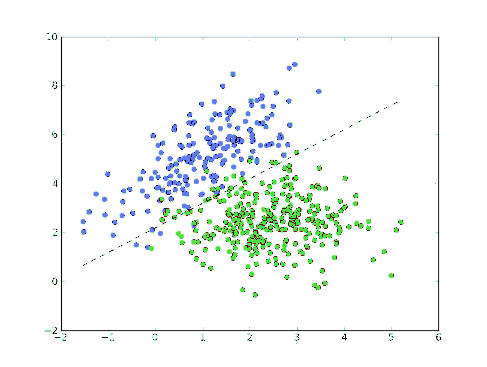
\includegraphics[scale=0.6]{ML-example.png}}}
\end{equation}

例如,在\emp{机器视觉}中,一张图像可以有几万个 pixels,每个 pixel 是一个\emp{维度},它的\emp{颜色}就是这个维度上的\emp{座标值}。 整个空间就是\emp{所有图像}的空间,\emp{每一点}是一个图像,这种空间的维数很高(维数就是一张图像的 pixels 个数)。 通常我们讲解时用 2 维或 3 维空间,读者们要运用想像力幻想一下很高维的情况。

在中学数学中有学过,一条\emp{直线}的方程是这形式的:
\begin{eqnarray}
& \mbox{\footnotesize \color{red}{constants}} \tikzmark{constants} \nonumber \\
\nonumber \\
& {\color{red}{a}} \tikzmark{constA} x \tikzmark{varX} + {\color{red}{b}} \tikzmark{constB} y \tikzmark{varY} + {\color{red}{c}} \tikzmark{constC} = 0 \\
\nonumber \\
& \mbox{\footnotesize variables} \tikzmark{variables} \nonumber
\begin{tikzpicture}[overlay,remember picture]
  \draw[red] (constants.center) +(-30pt,-4pt) -- ([shift={(-3pt,8pt)}]constA.center);
  \draw[red] (constants.center) +(-20pt,-4pt) -- ([shift={(-1pt,10pt)}]constB.center);
  \draw[red] (constants.center) +(-10pt,-4pt) -- ([shift={(-1pt,8pt)}]constC.center);
  \draw (variables.center) +(-29pt,8pt) -- ([shift={(-4pt,-2pt)}]varX.center);
  \draw (variables.center) +(-15pt,8pt) -- ([shift={(-4pt,-4pt)}]varY.center);
\end{tikzpicture}
\end{eqnarray}

它的\emp{几何}解释是这样的:
\begin{equation}
\vcenter{\hbox{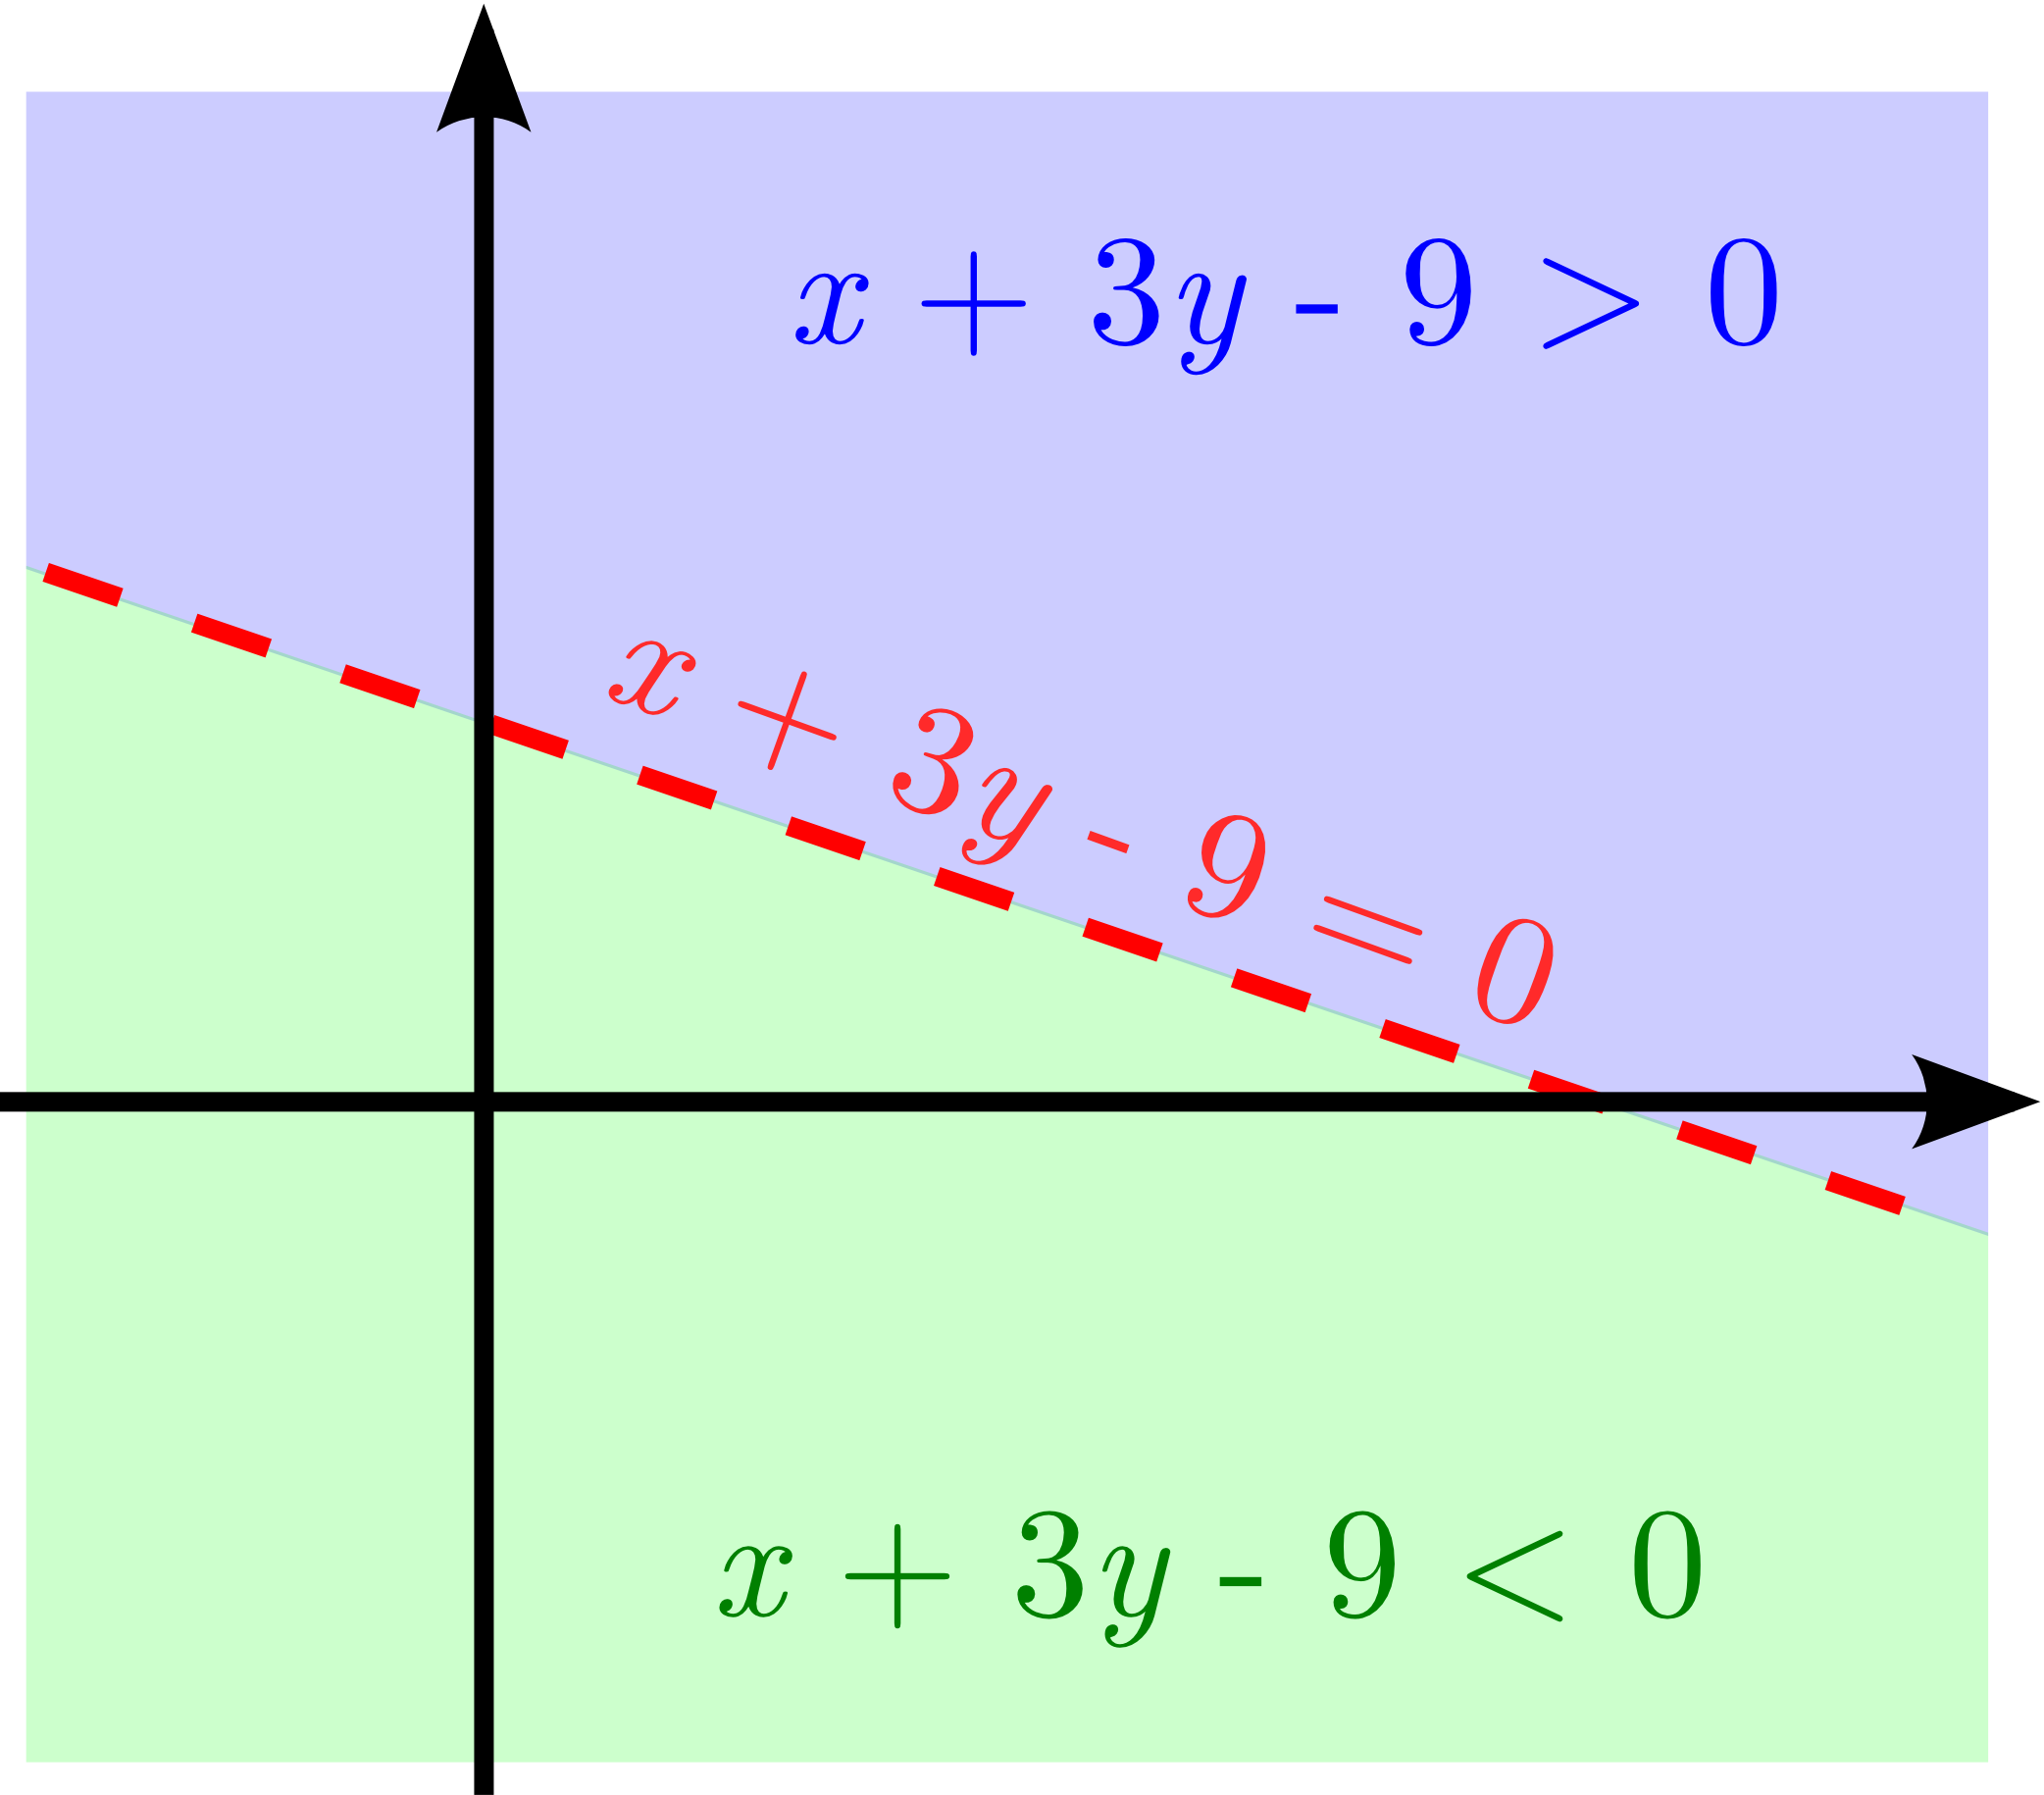
\includegraphics[scale=0.75]{linear-inequality.png}}}
\end{equation}
在直线上,那直线的方程 $= 0$。 直线将它身在的空间\emp{分割}成两半: 一边 $> 0$,另一边 $< 0$。

推广到 3 维空间的情况,我们有一个\emp{平面}的方程: 
\begin{equation}
{\color{red}{a}}x + {\color{red}{b}}y + {\color{red}{c}}z + {\color{red}{d}} = 0
\end{equation}
它同样将空间\emp{分割}成两半,一半 $> 0$,另一半 $< 0$:
\begin{equation}
\vcenter{\hbox{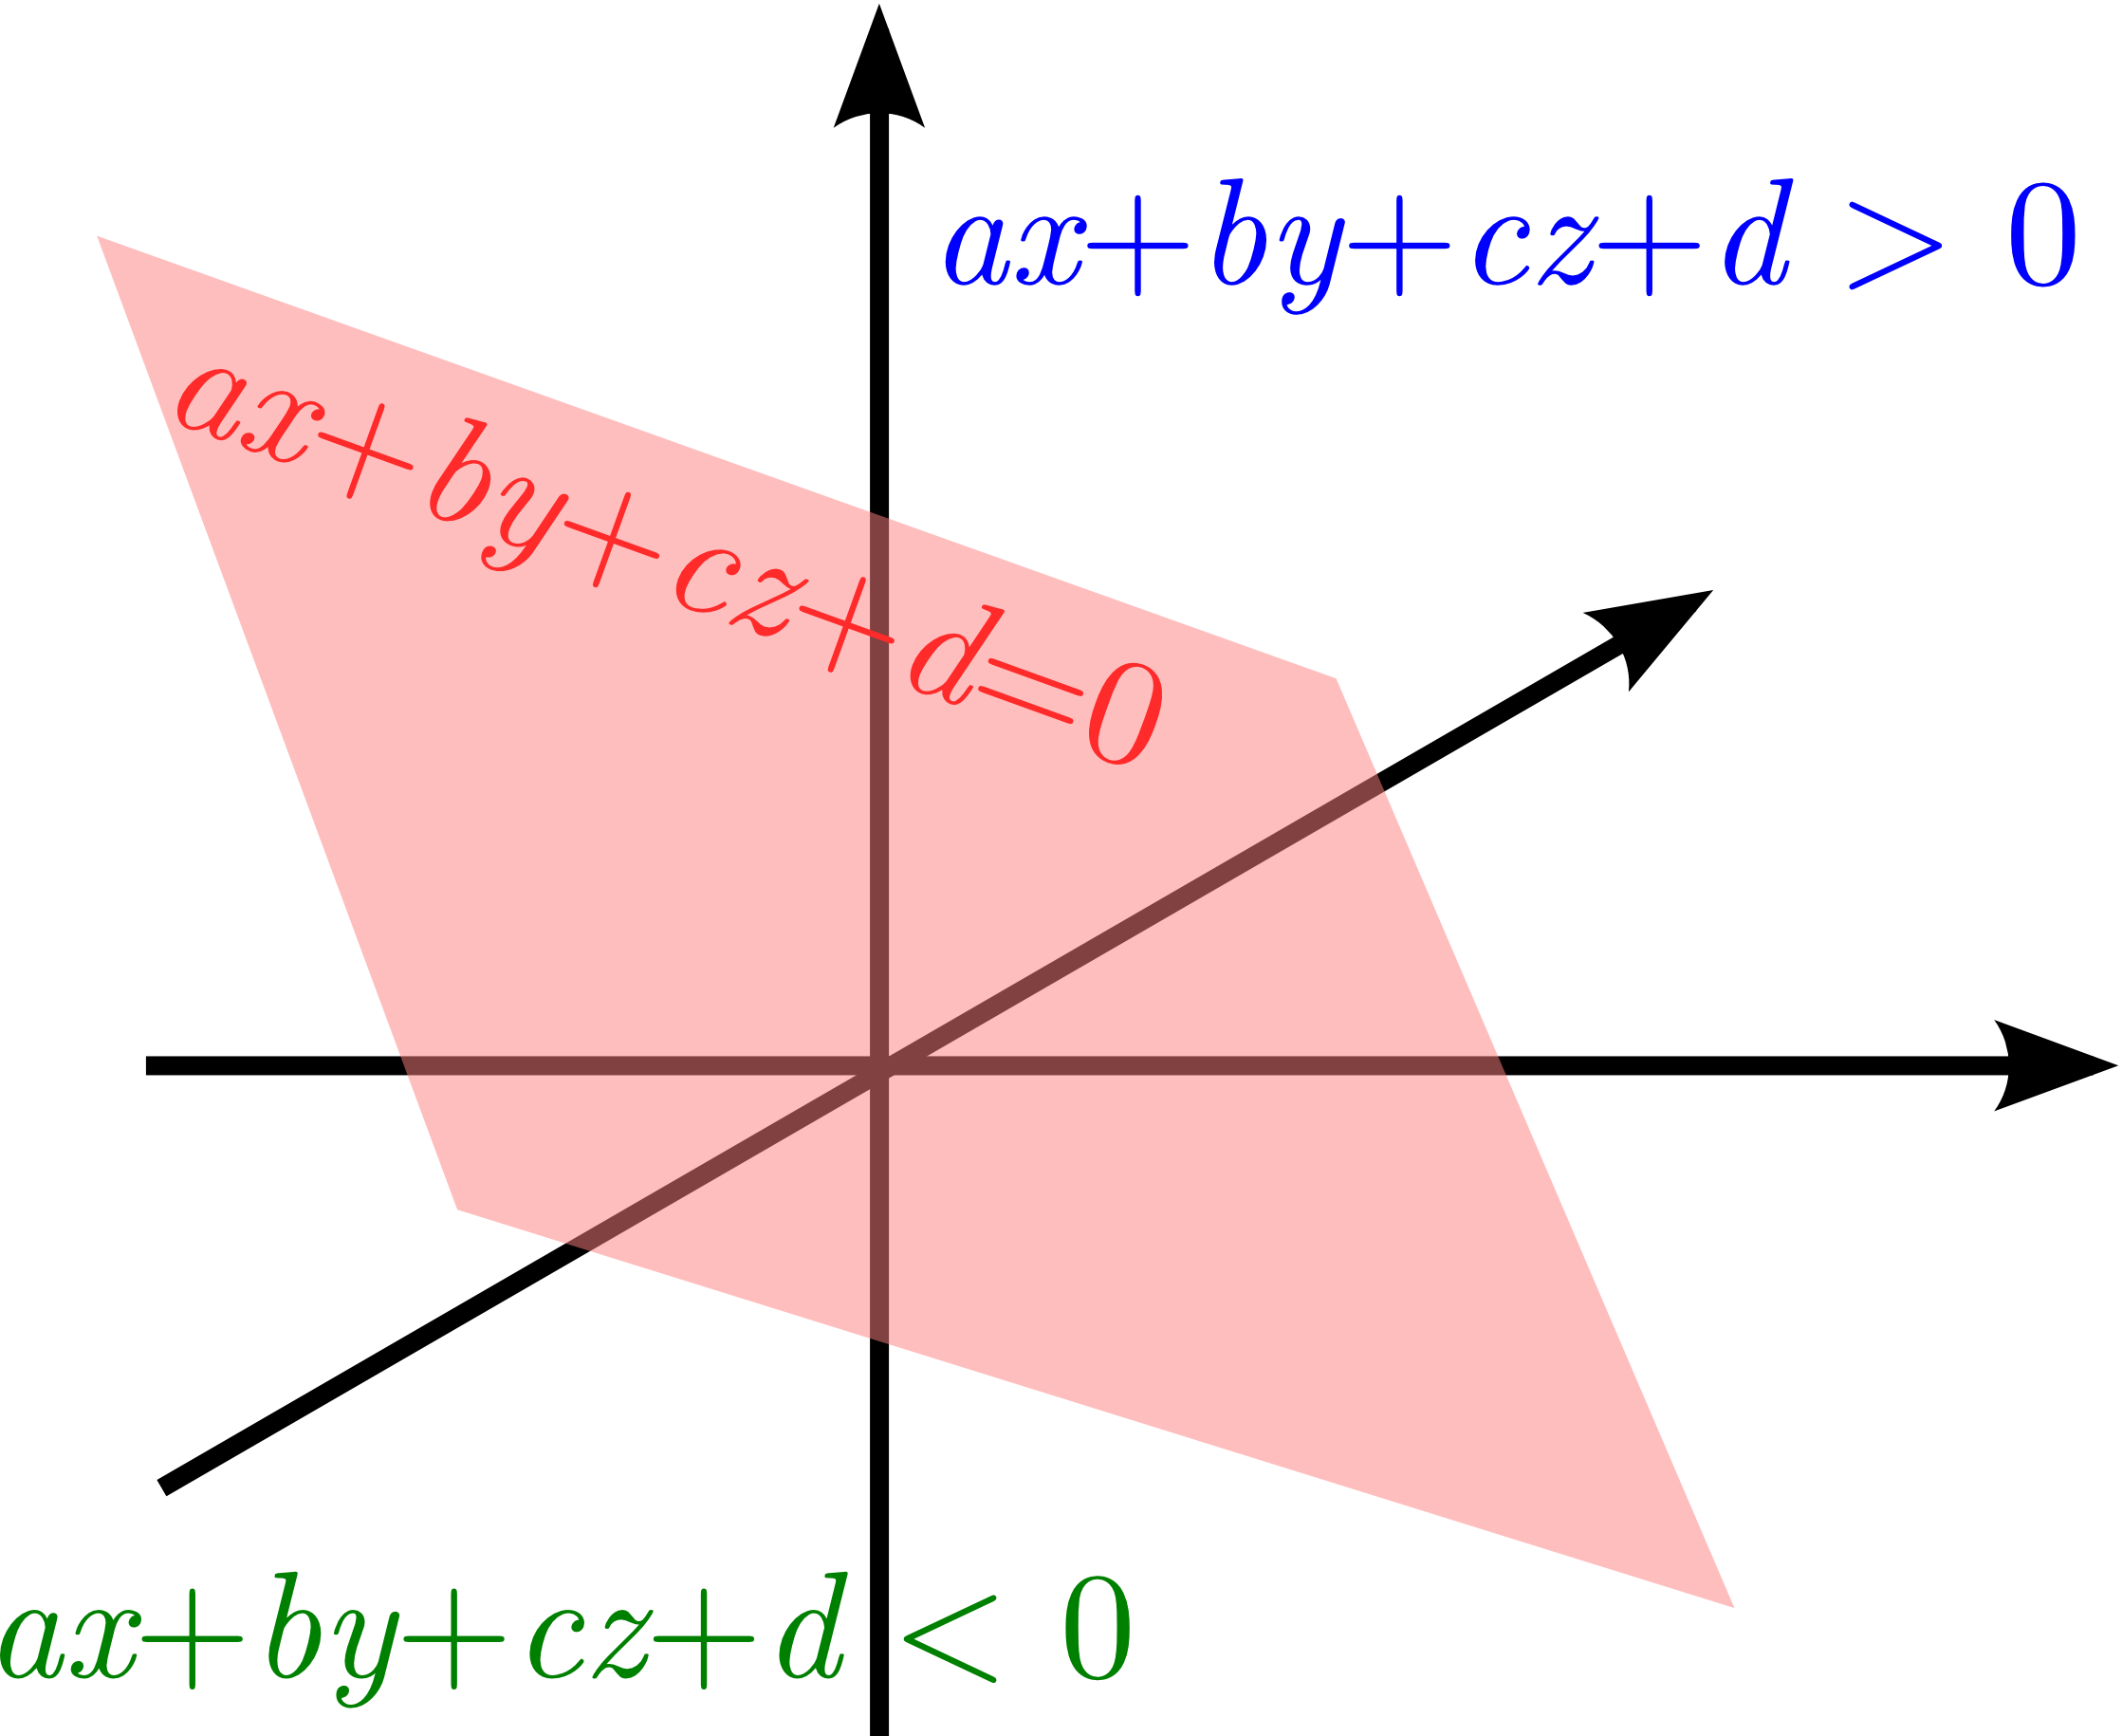
\includegraphics[scale=0.75]{linear-inequality-2.png}}}
\end{equation}

在任意 $n$-维空间,每一点记作 $\vect{x} = (x_1, x_2, ..., x_n)$,一个\emp{超平面} (hyper-plane) 将该空间分割成两半,它的方程是: 
\begin{equation}
{\color{red}{a_1}}x_1 + {\color{red}{a_2}}x_2 + .... + {\color{red}{a_n}}x_n + {\color{red}{a_0}} = 0
\label{eqn:general-linear}
\end{equation}

\begin{tcolorbox}[colback=lightyellow, breakable, enhanced]
注意: 一块超平面的维数是多少? 在平面空间里它是一条线(1 度空间),在立体空间里它是平面(2 度空间), 一般来说,在 $n$-维空间里的超平面是一个 $n - 1$ 维的物体,$(n-1)$ 又叫作 co-dimension 1,意思是说 ambient space 的维数是 $n$,方程 (\ref{eqn:general-linear}) 减少了一个\emp{自由度} (degree of freedom),所以\emp{服从}这等式的物体内,只有 $n - 1$ 个自由度。 
\end{tcolorbox}

现在可以看到超平面和神经元之间有些相似,因为神经元在未经过 $\sigmoid$ 之前,就是一个 \emp{线性组合}: 
\begin{eqnarray}
& \mbox{\footnotesize \color{red}{linear combination}} \nonumber \\
\boxed{output} \; y = \sigmoid & [ \; \overbrace{\sum_i (w_i \; x_i)} \; ]
\end{eqnarray}
换句话说: \uline{每粒神经元构成一超平面,它将空间切割成两半}。

加了 $\sigmoid$ 之后怎样? 未有 $\sigmoid$ 时,分割的两边分别是 $> 0$ 和 $< 0$,如果将颜色看作是「强度」,强度是逐渐变化的:  (右边表示从侧面看,立体)
\begin{equation}
\vcenter{\hbox{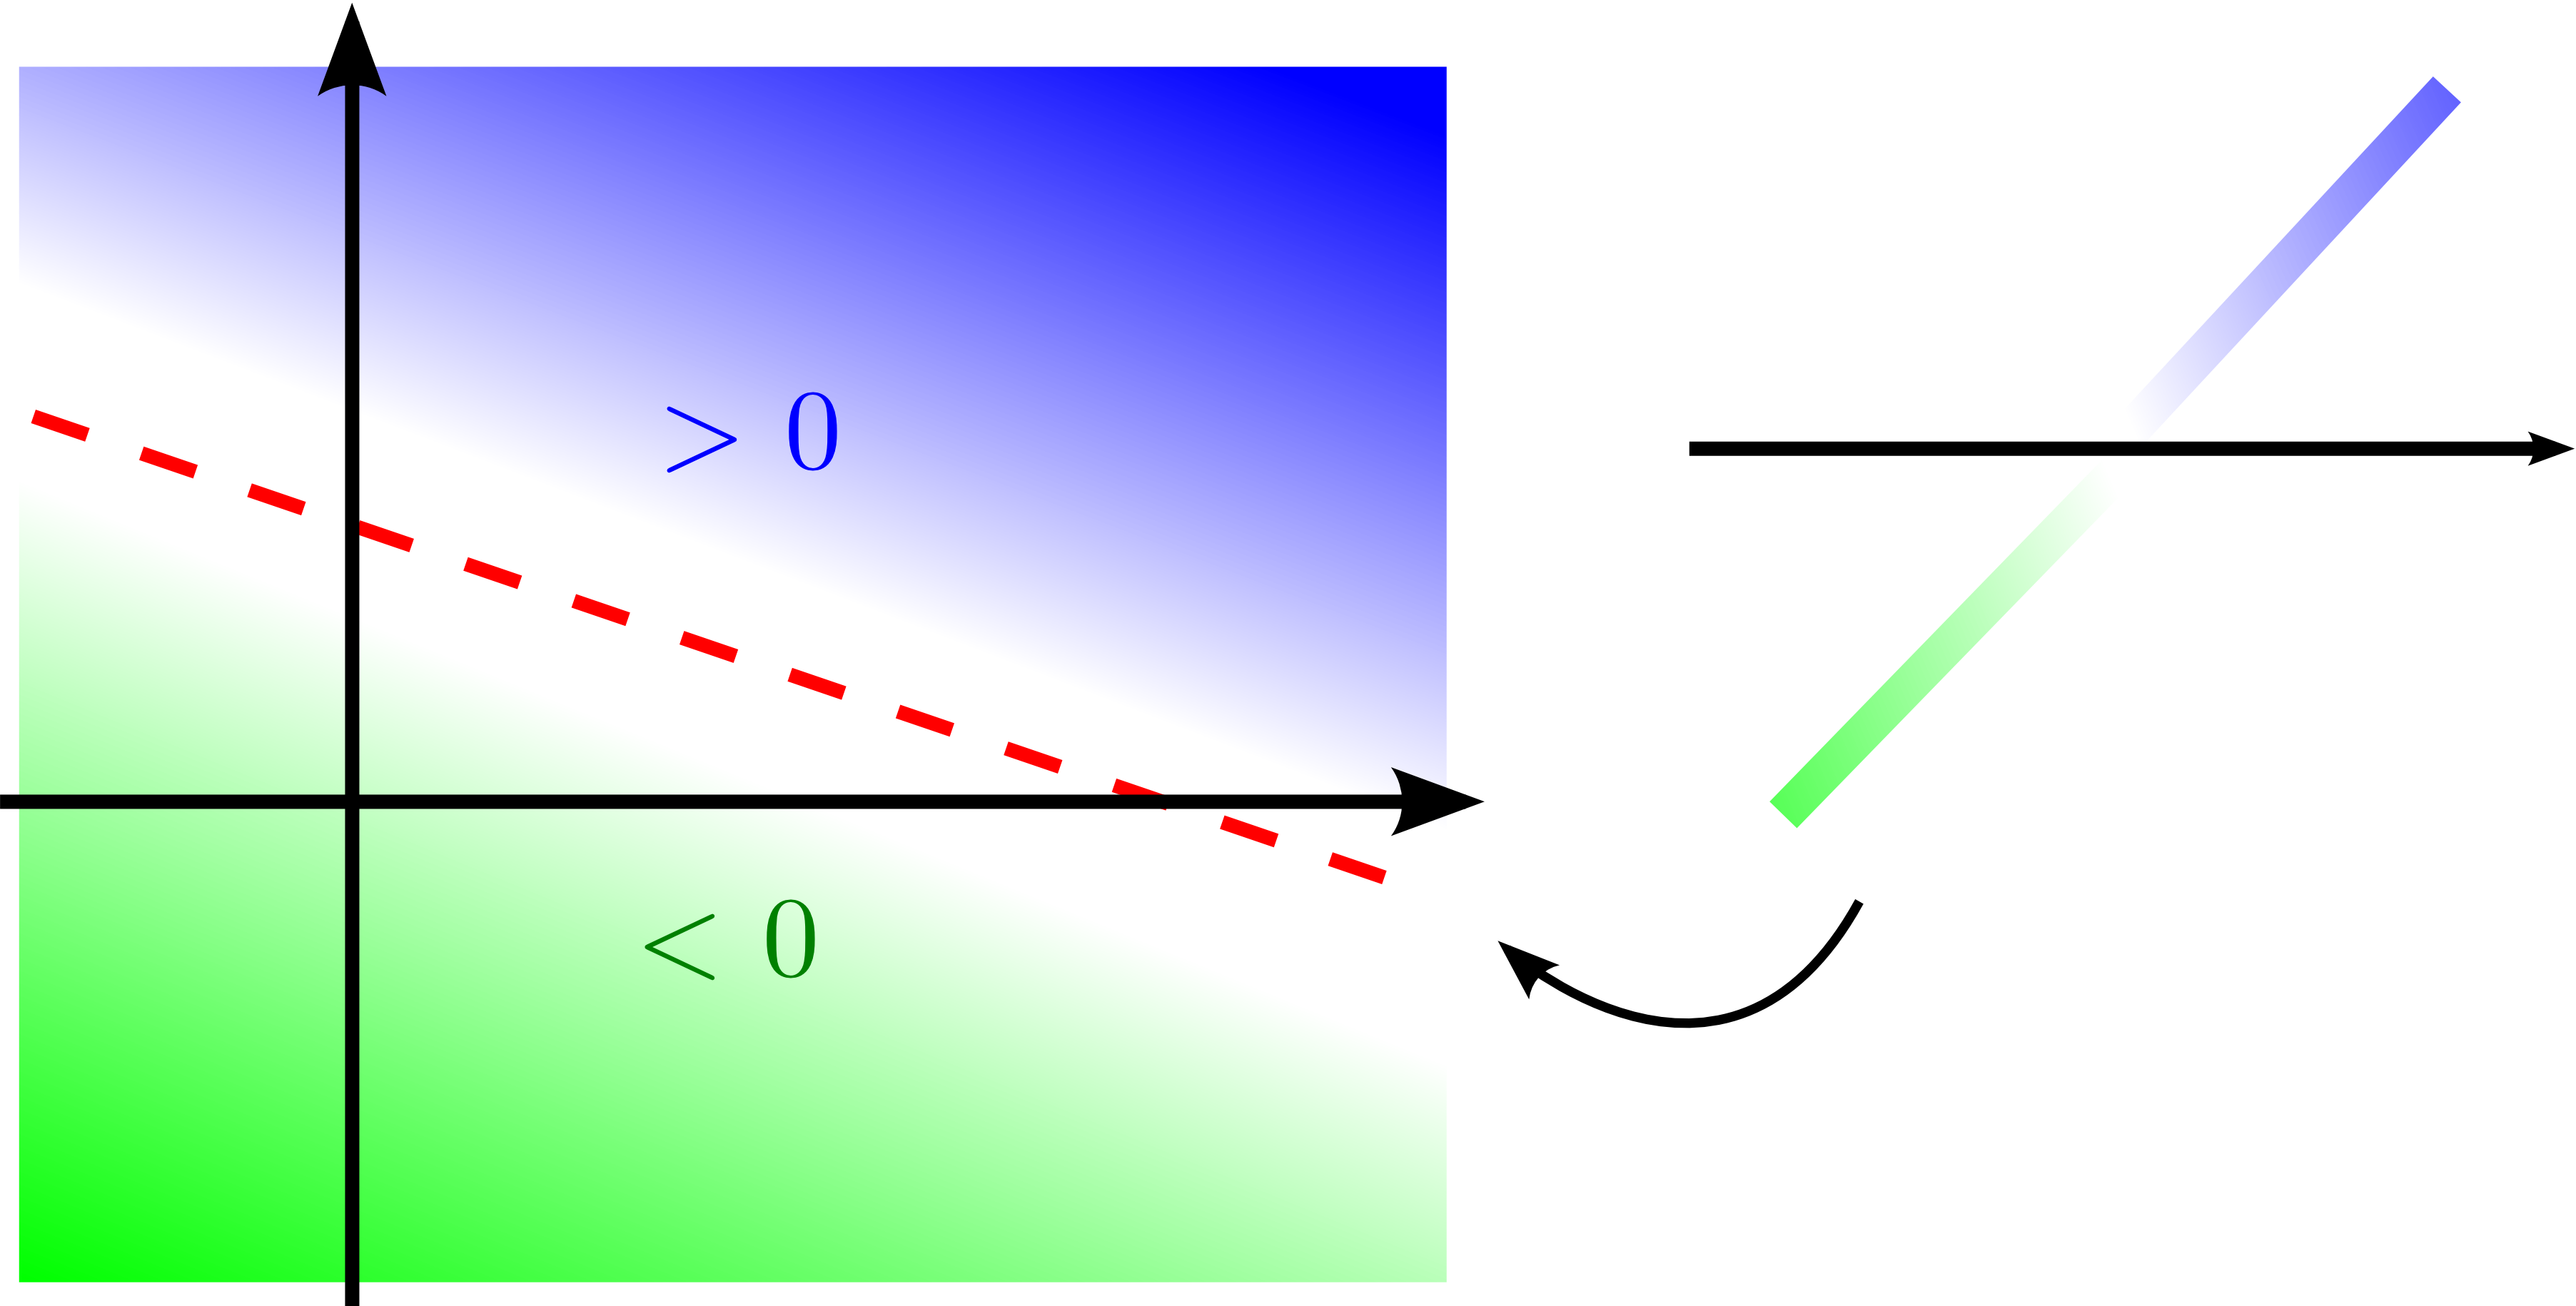
\includegraphics[scale=0.6]{linear-inequality-3.png}}}
\end{equation}
加了 sigmoid 之后,用 1 代表「yes」,0 代表「no」,则两边的对比加强了,亦即更\emp{两极化}、「非此即彼」:
\begin{equation}
\vcenter{\hbox{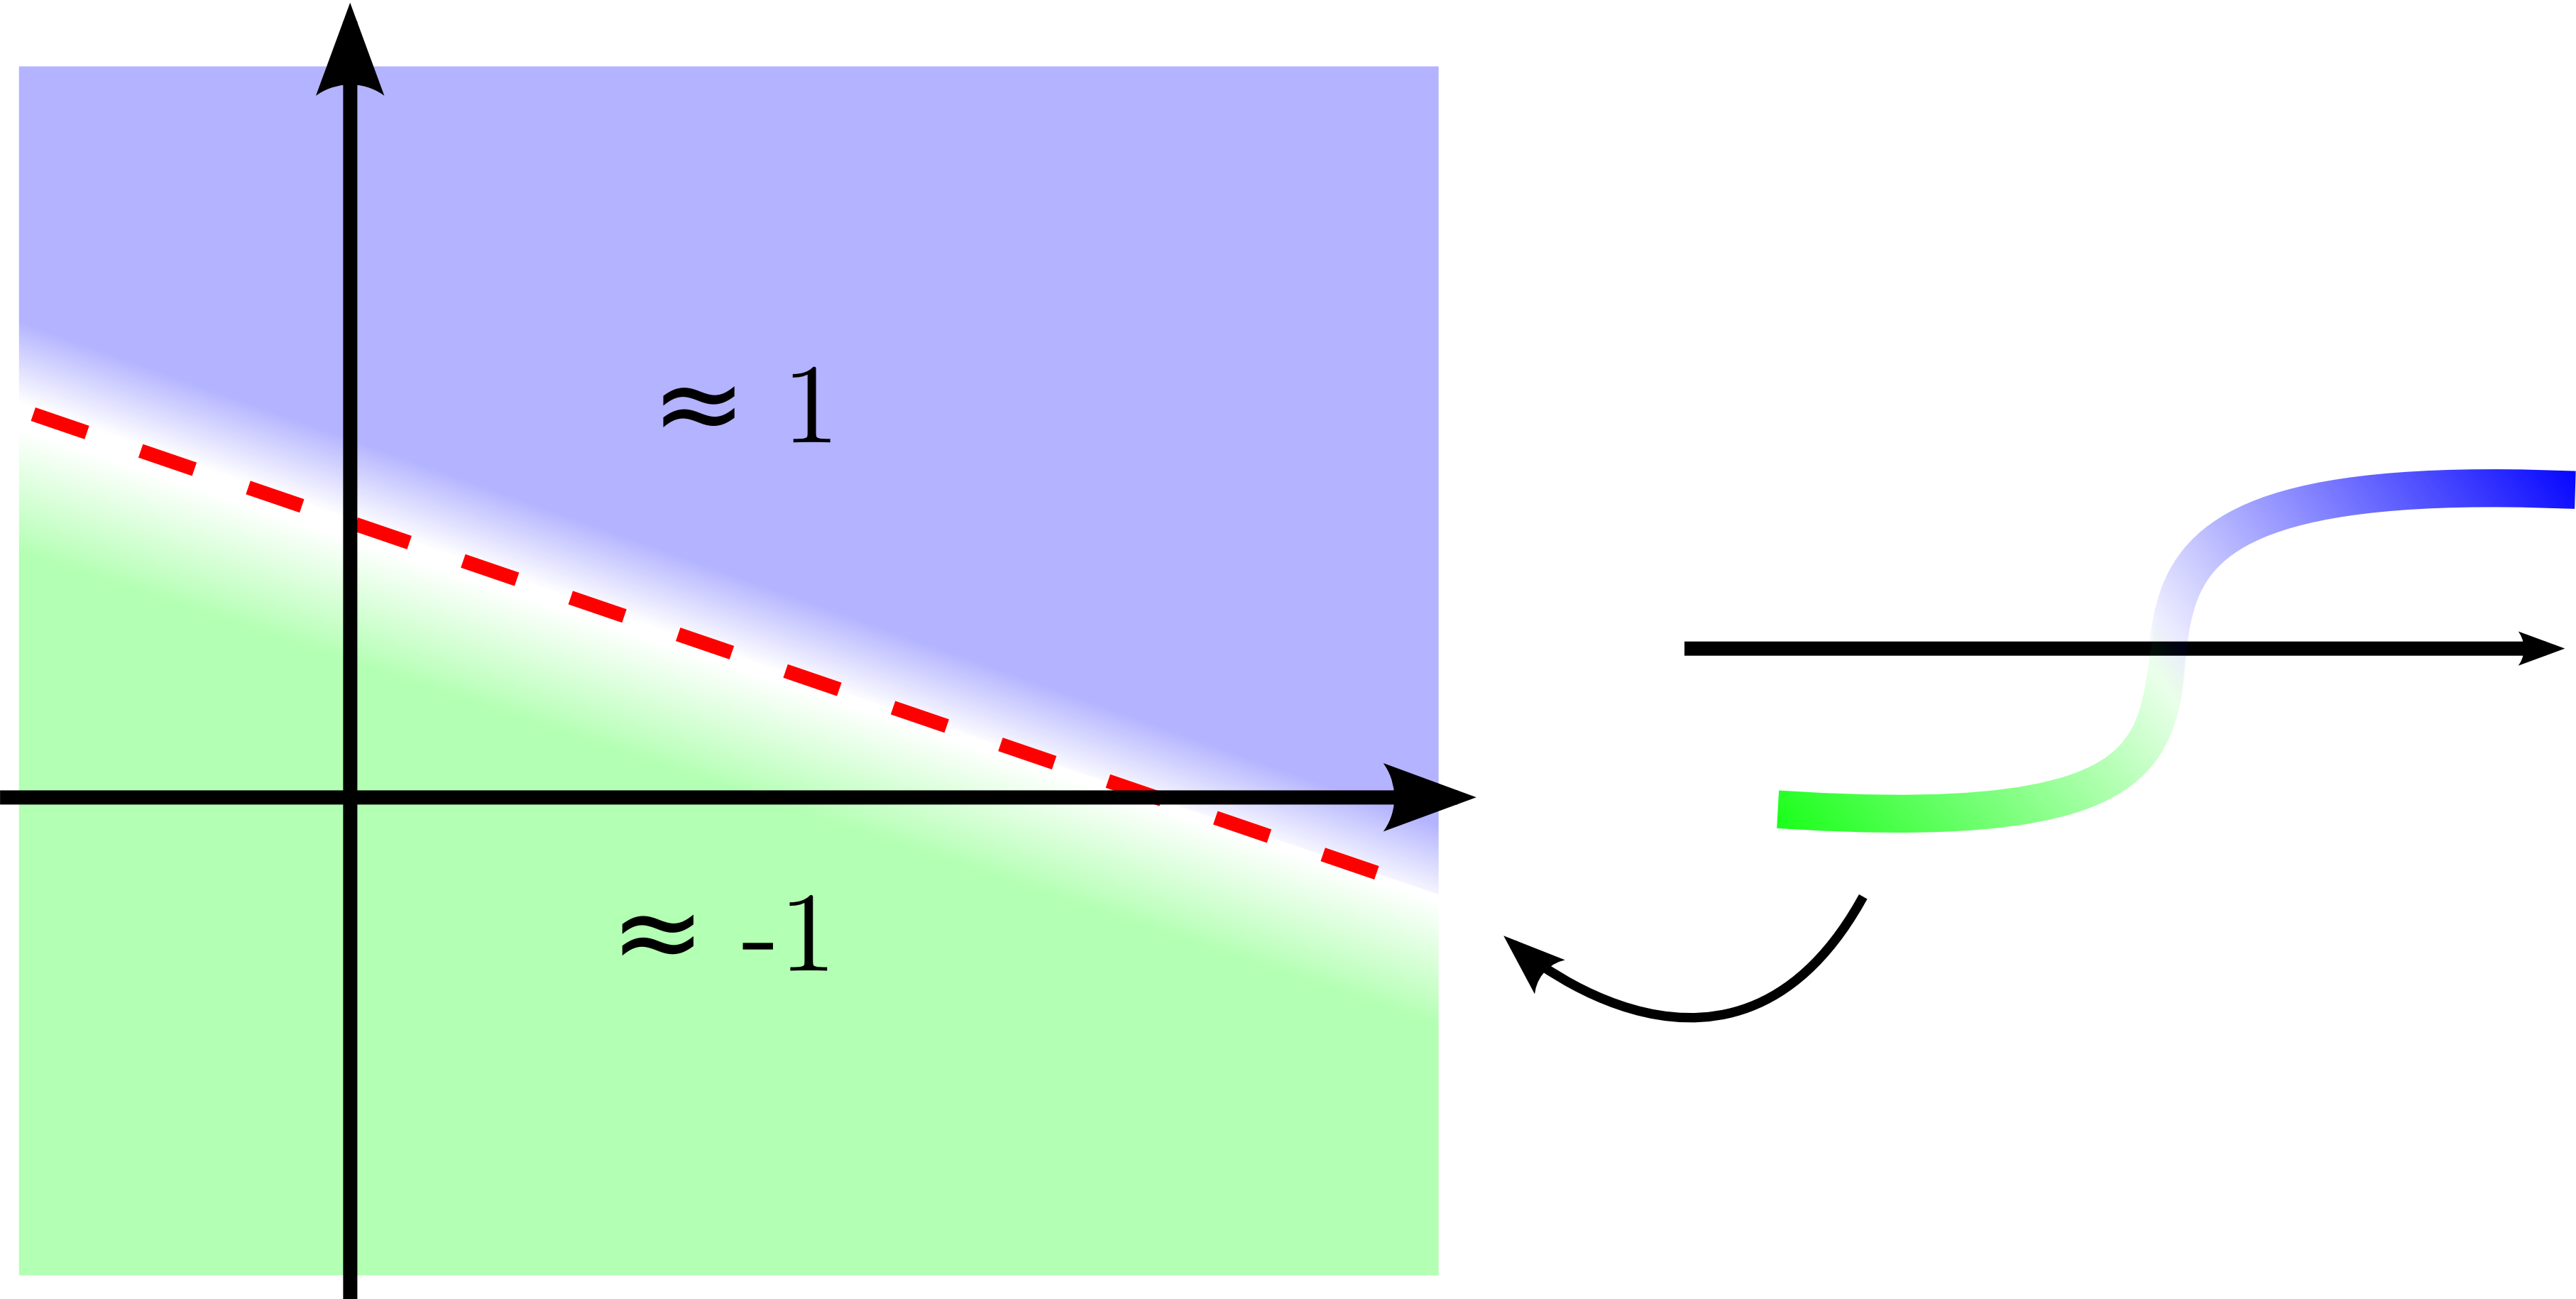
\includegraphics[scale=0.6]{linear-inequality-4.png}}}
\end{equation}

\section*{> 1 粒神经元}

如果有 $> 1$ 粒神经元(在同一层上),例如 3 粒:
\begin{equation}
\vcenter{\hbox{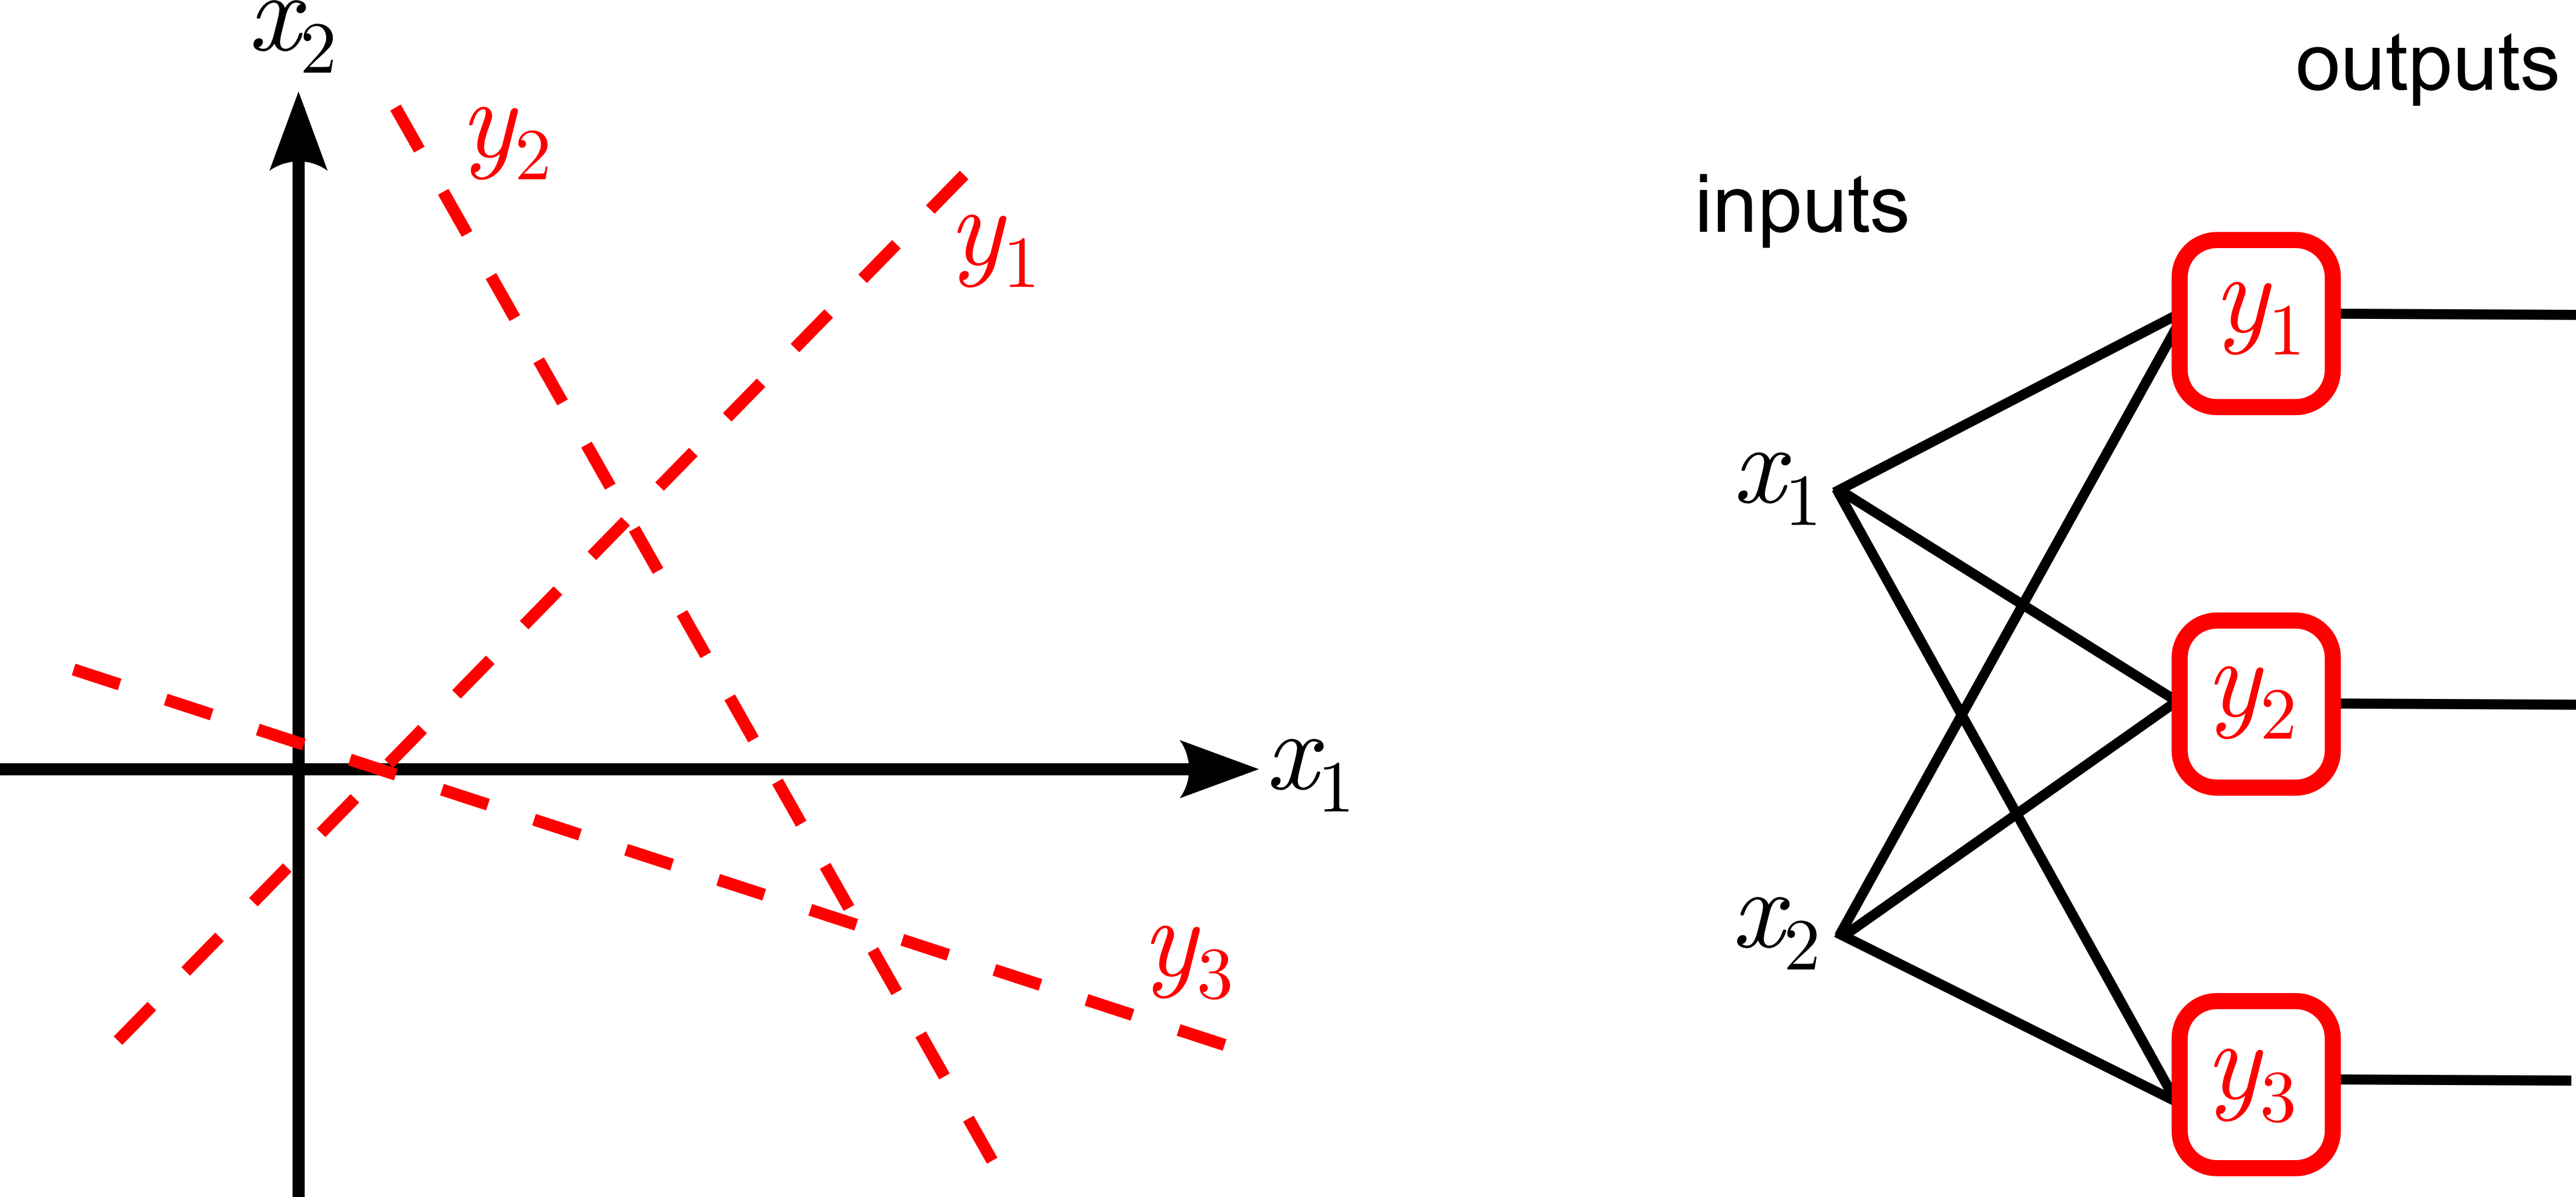
\includegraphics[scale=0.6]{linear-inequalities-1.png}}}
\label{simple-network-layer}
\end{equation}
注意: 座标是 $(x_1, x_2) = $ 输入,输出是 $(y_1, y_2, y_3)$,分别用 3 条{\color{red}{虚线}}代表。 这\emp{一层}神经网络的 network topology 如 (\ref{simple-network-layer}) 右图所示(每粒神经元没有画出 $\sum$ 和 $\sigmoid$)。

每粒神经元可以选择某一边为「yes」,这些选择的 conjunction 可以形成不同的形状,例如以下两种: 
\begin{equation}
\vcenter{\hbox{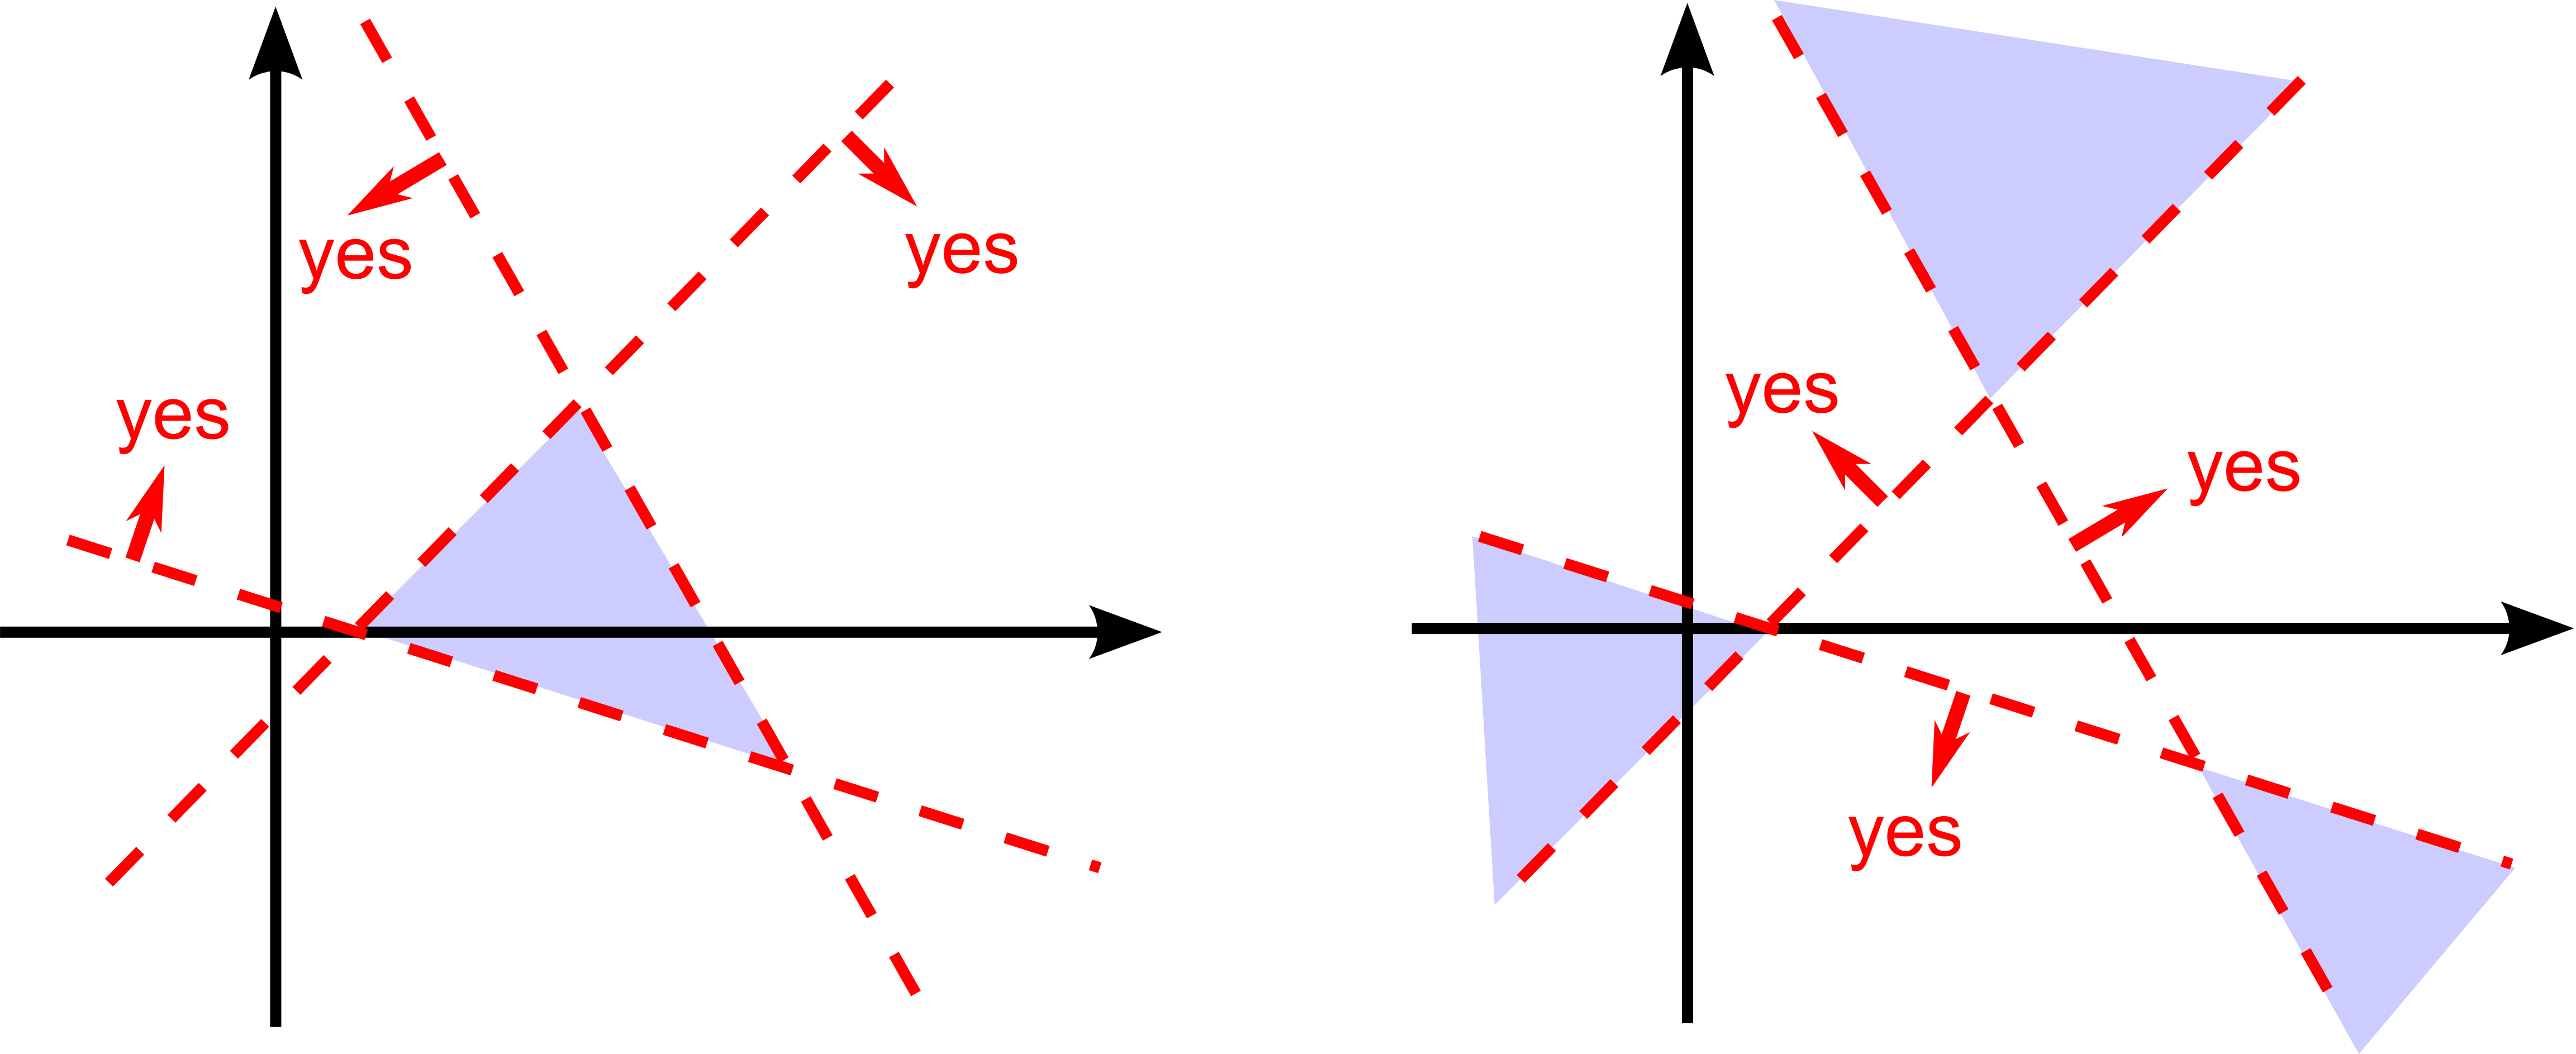
\includegraphics[scale=0.6]{linear-inequalities-2.png}}}
\end{equation}
亦注意在右图中,可以出现几个 disjoint regions(在空间上分离的)。

很明显,可以用神经元将输入空间的点进行切割和分类,达到\emp{机器学习}的目的。

\section*{一层神经网络}

%简单来说,当神经网络的\emp{层数}增加,在输入空间的切割形状会变得更为\emp{复杂},所以多层的神经网络有能力学习出非常复杂的 patterns,这就是\emp{深度学习}的优势。

接下来要用到更多 \emp{线性代数},我会在另一篇 tutorial 解释。 

一层神经网络的数学形式是:
\begin{equation}
\boxed{output} \; \vect{y} = \sigmoid [ W \vect{x} ] 
\end{equation}
其中 $W$ 是矩阵,亦即 \emp{线性变换}; $\sigmoid$ 是 \emp{非线性变换}。

矩阵是 \emp{线性方程组} 的紧凑写法。 一粒神经元 = $\sigmoid \circ \boxed{线性组合}$,一条线性组合是矩阵中的一行。

每一个矩阵都代表一个 \emp{linear transformation}:
\begin{equation}
\vcenter{\hbox{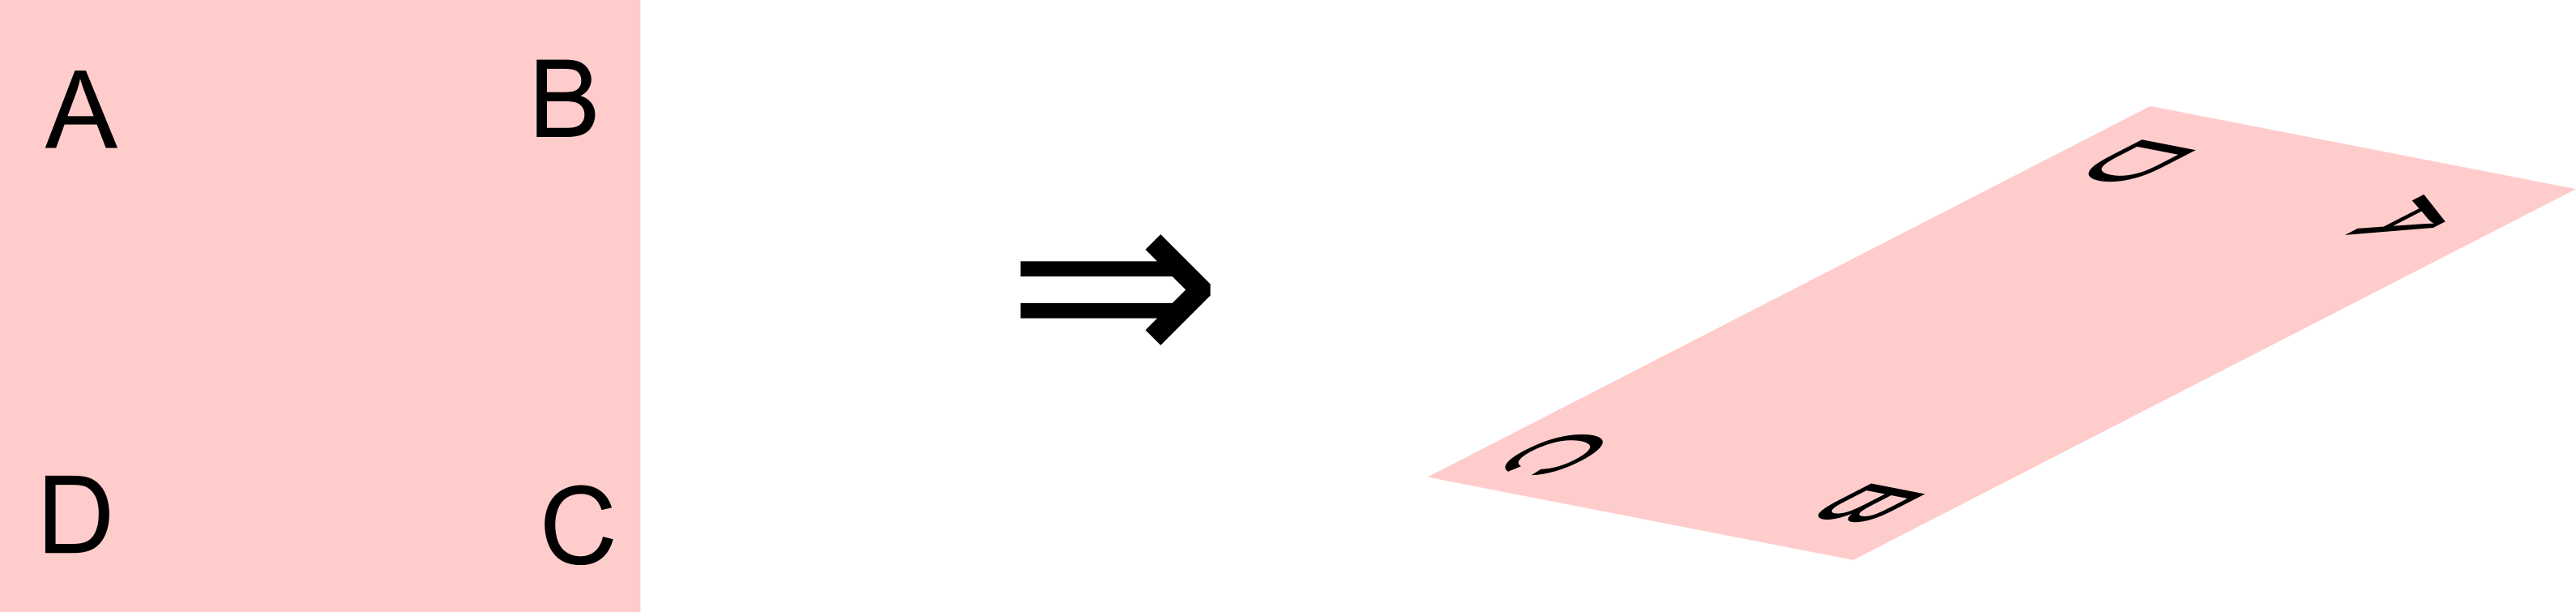
\includegraphics[scale=0.6]{linear-transformation.png}}}
\end{equation}
线性变换可以将正方形「扯」成平行四边形,也包括位置上的\emp{旋转} (rotation) 和\emp{平移} (translation)。 但直线仍变为直线,故名。

另外要明白 $\sigmoid$ 变换的形状: (以下是 $x$ 和 $y$ 座标都被 sigmoid 变换)
\begin{equation}
\vcenter{\hbox{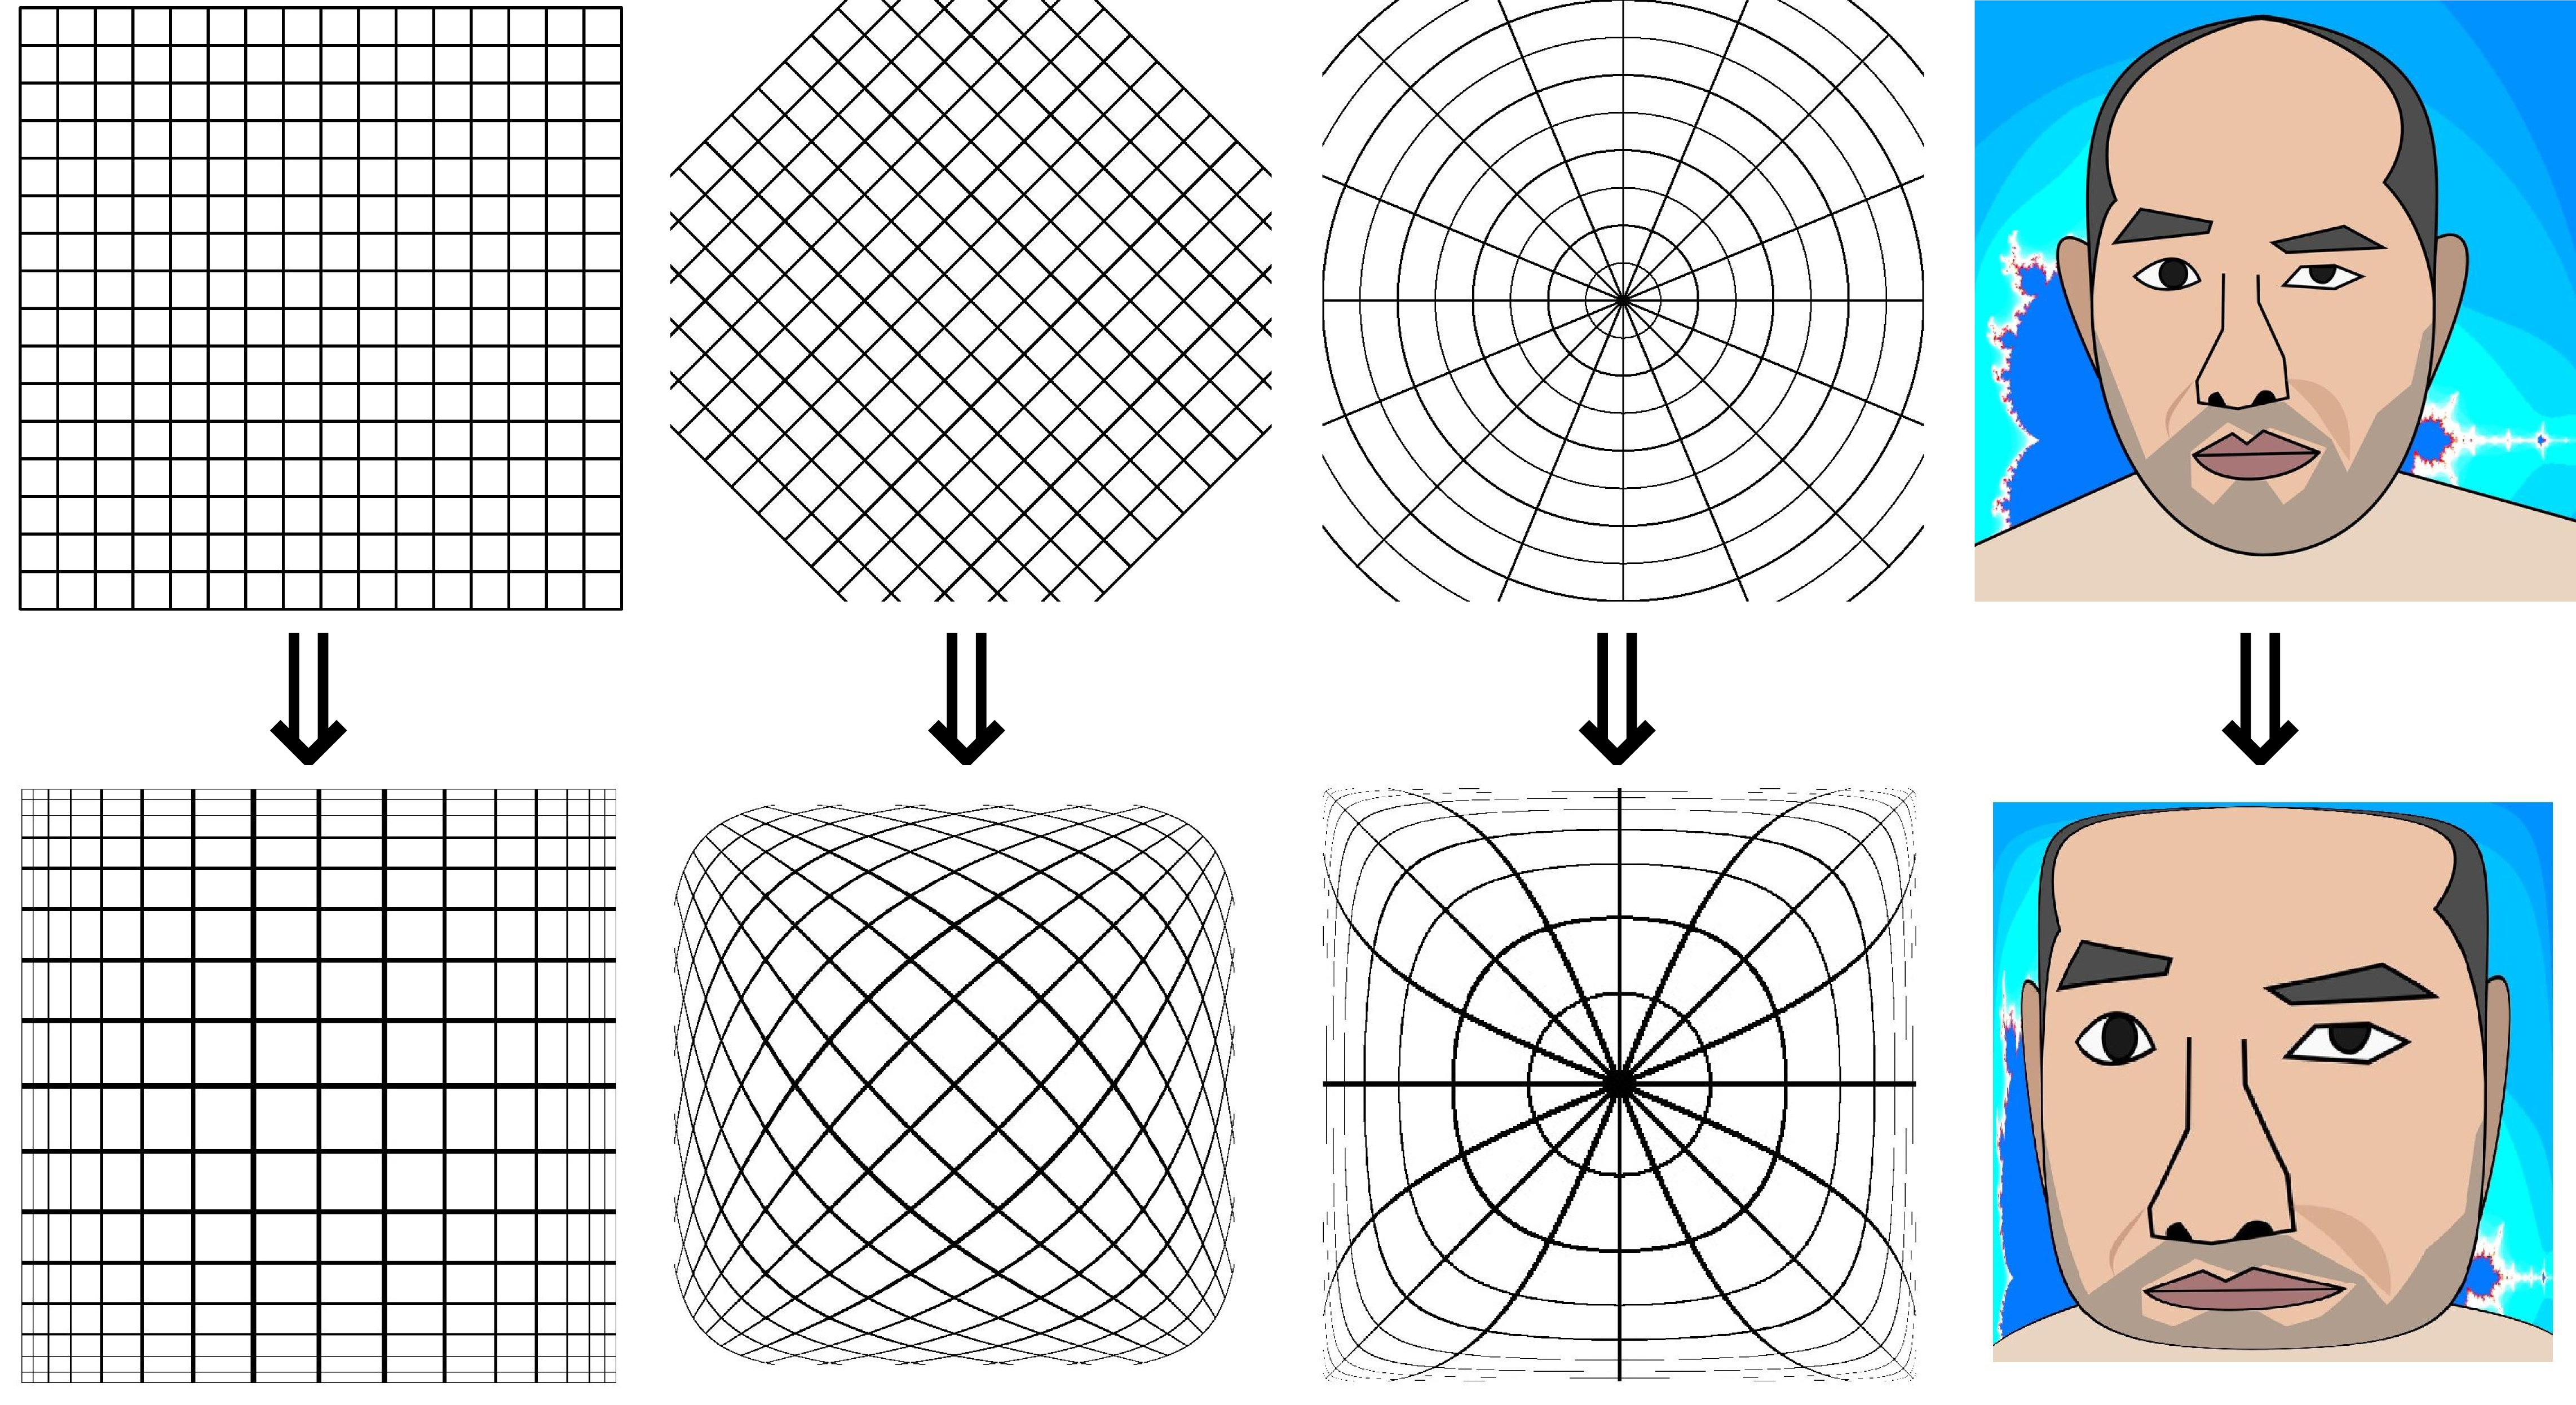
\includegraphics[scale=0.75]{sigmoid-transforms.png}}}
\end{equation}
可以这样理解 $\sigmoid$: 它将平面上的点「扯向」4个角位,,所以我变了「国字口面」。

我们说这些顶点是\emp{吸引子} (attractors):
\begin{equation}
\vcenter{\hbox{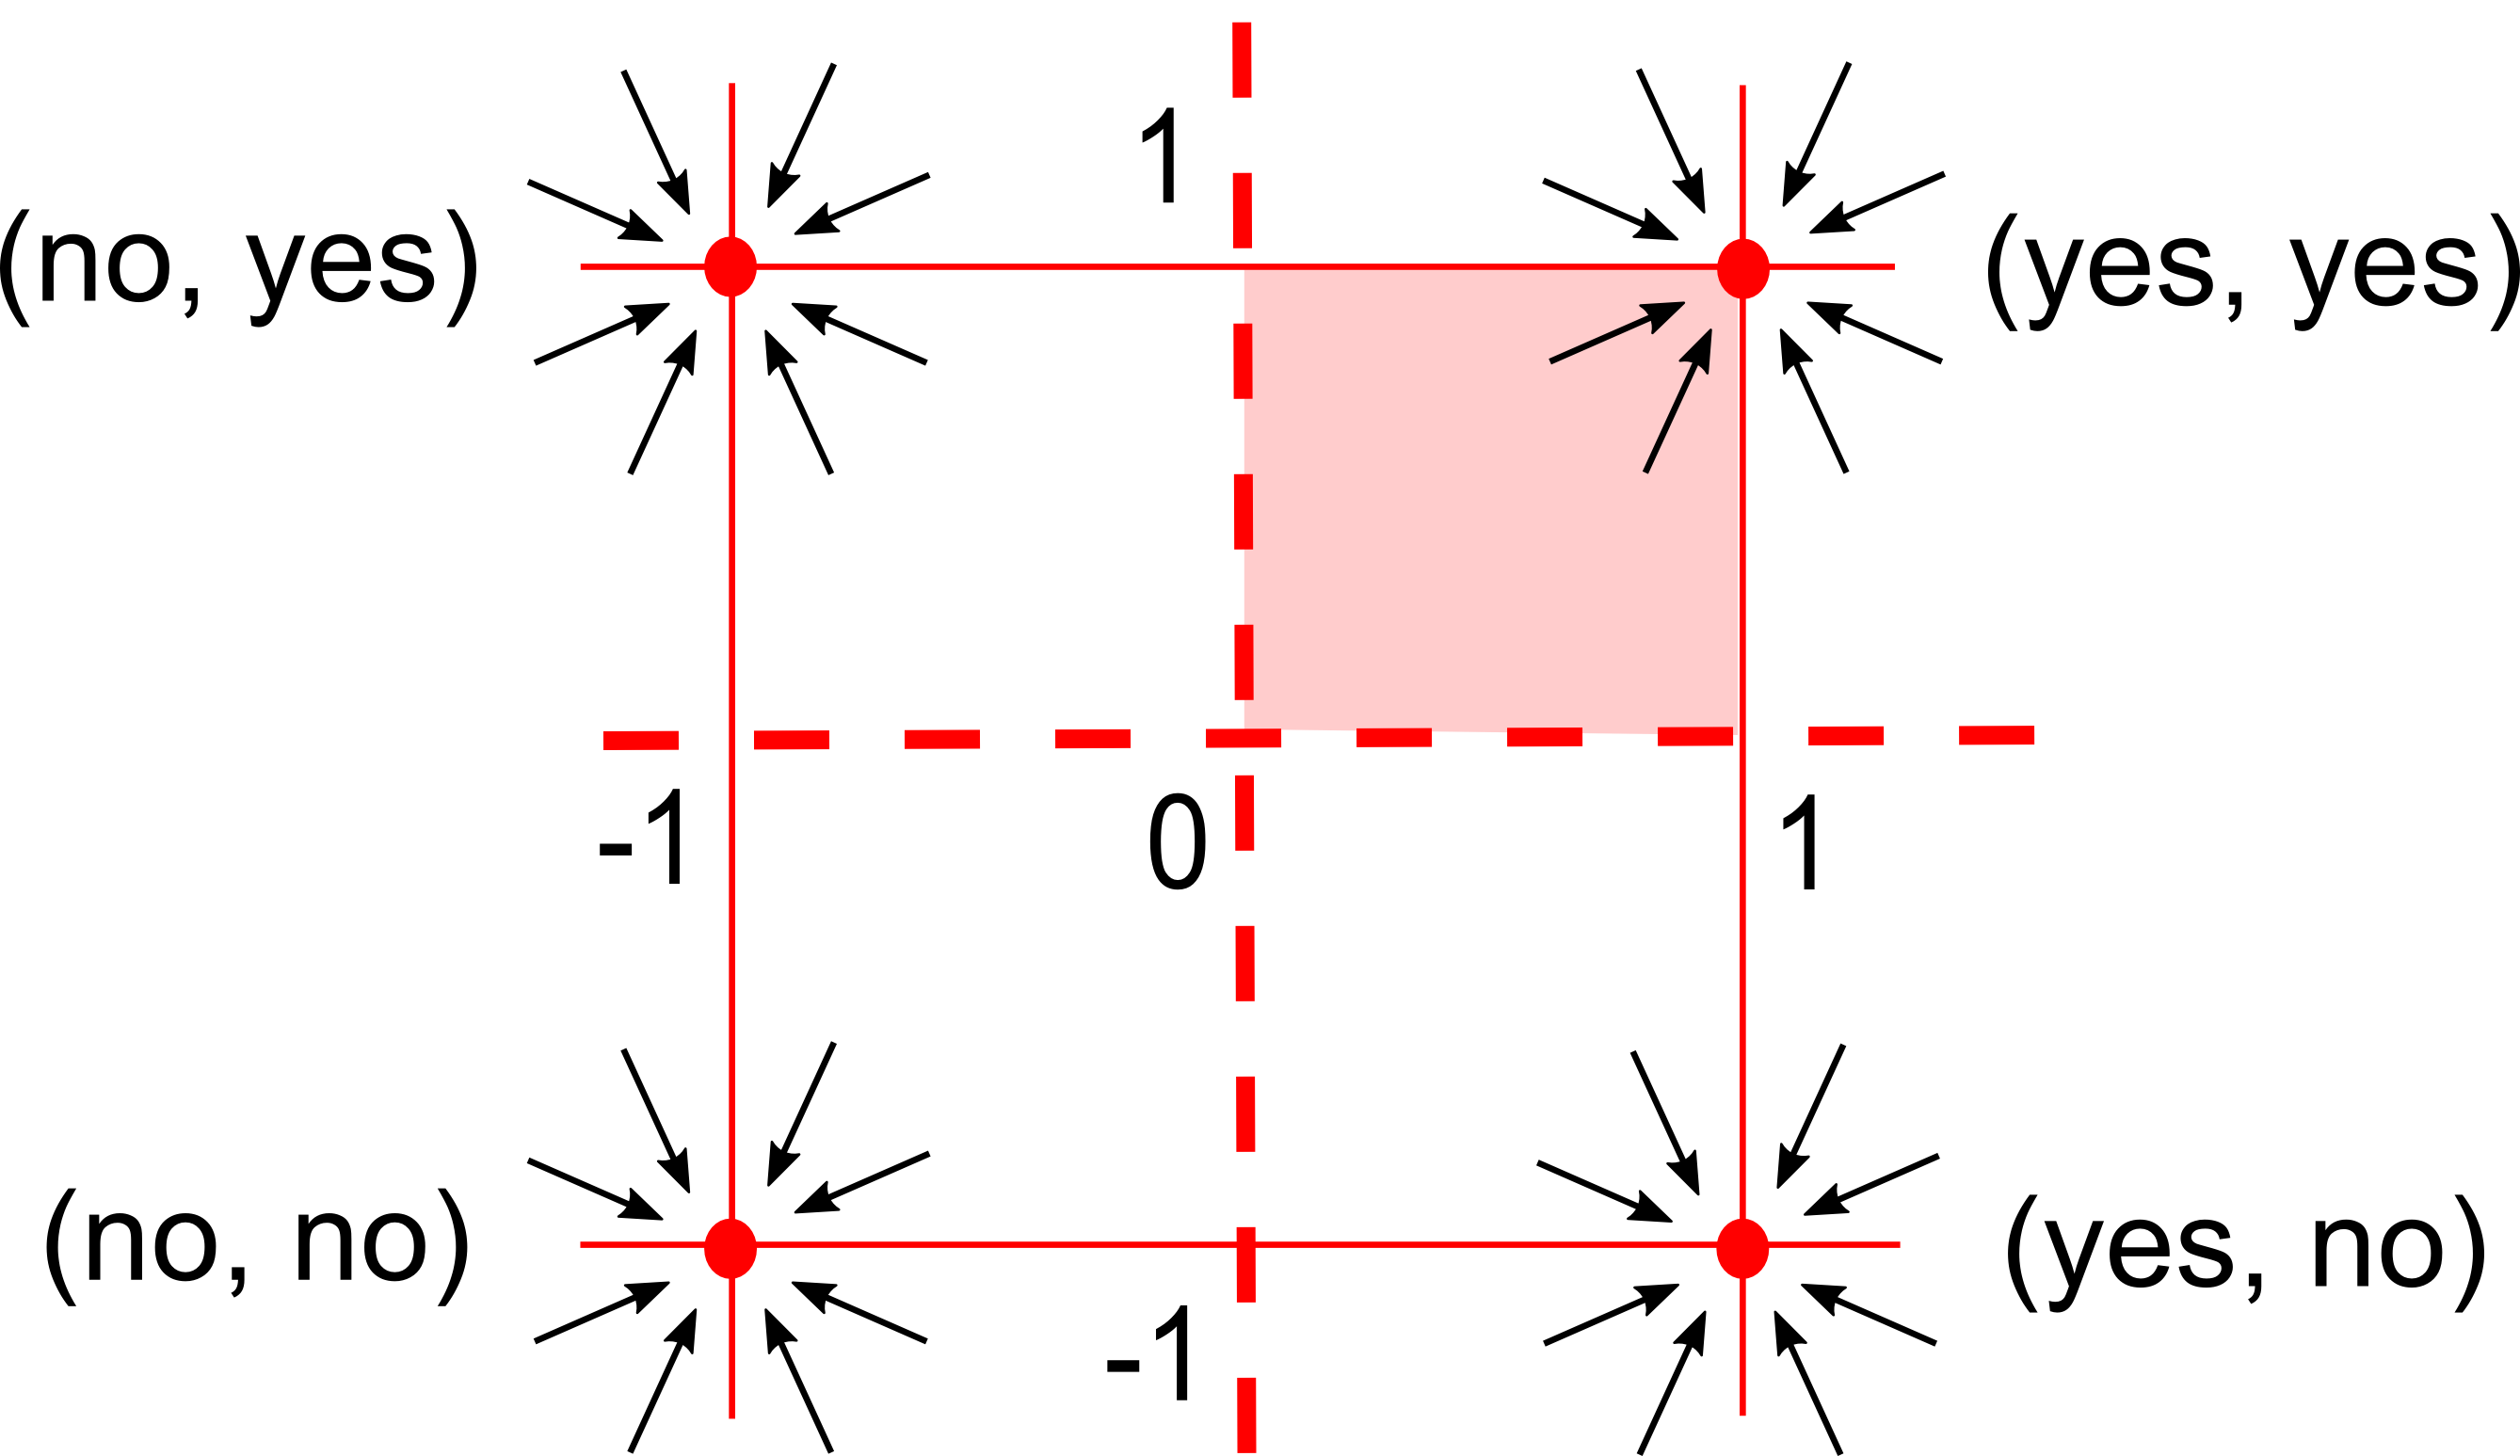
\includegraphics[scale=0.75]{attractors.png}}}
\end{equation}

注意: 在 $\sigmoid$ 变换时,图像是从周围\emp{无限}的空间压缩到 $[-1,+1]^2$ 这方格里:
\begin{equation}
\vcenter{\hbox{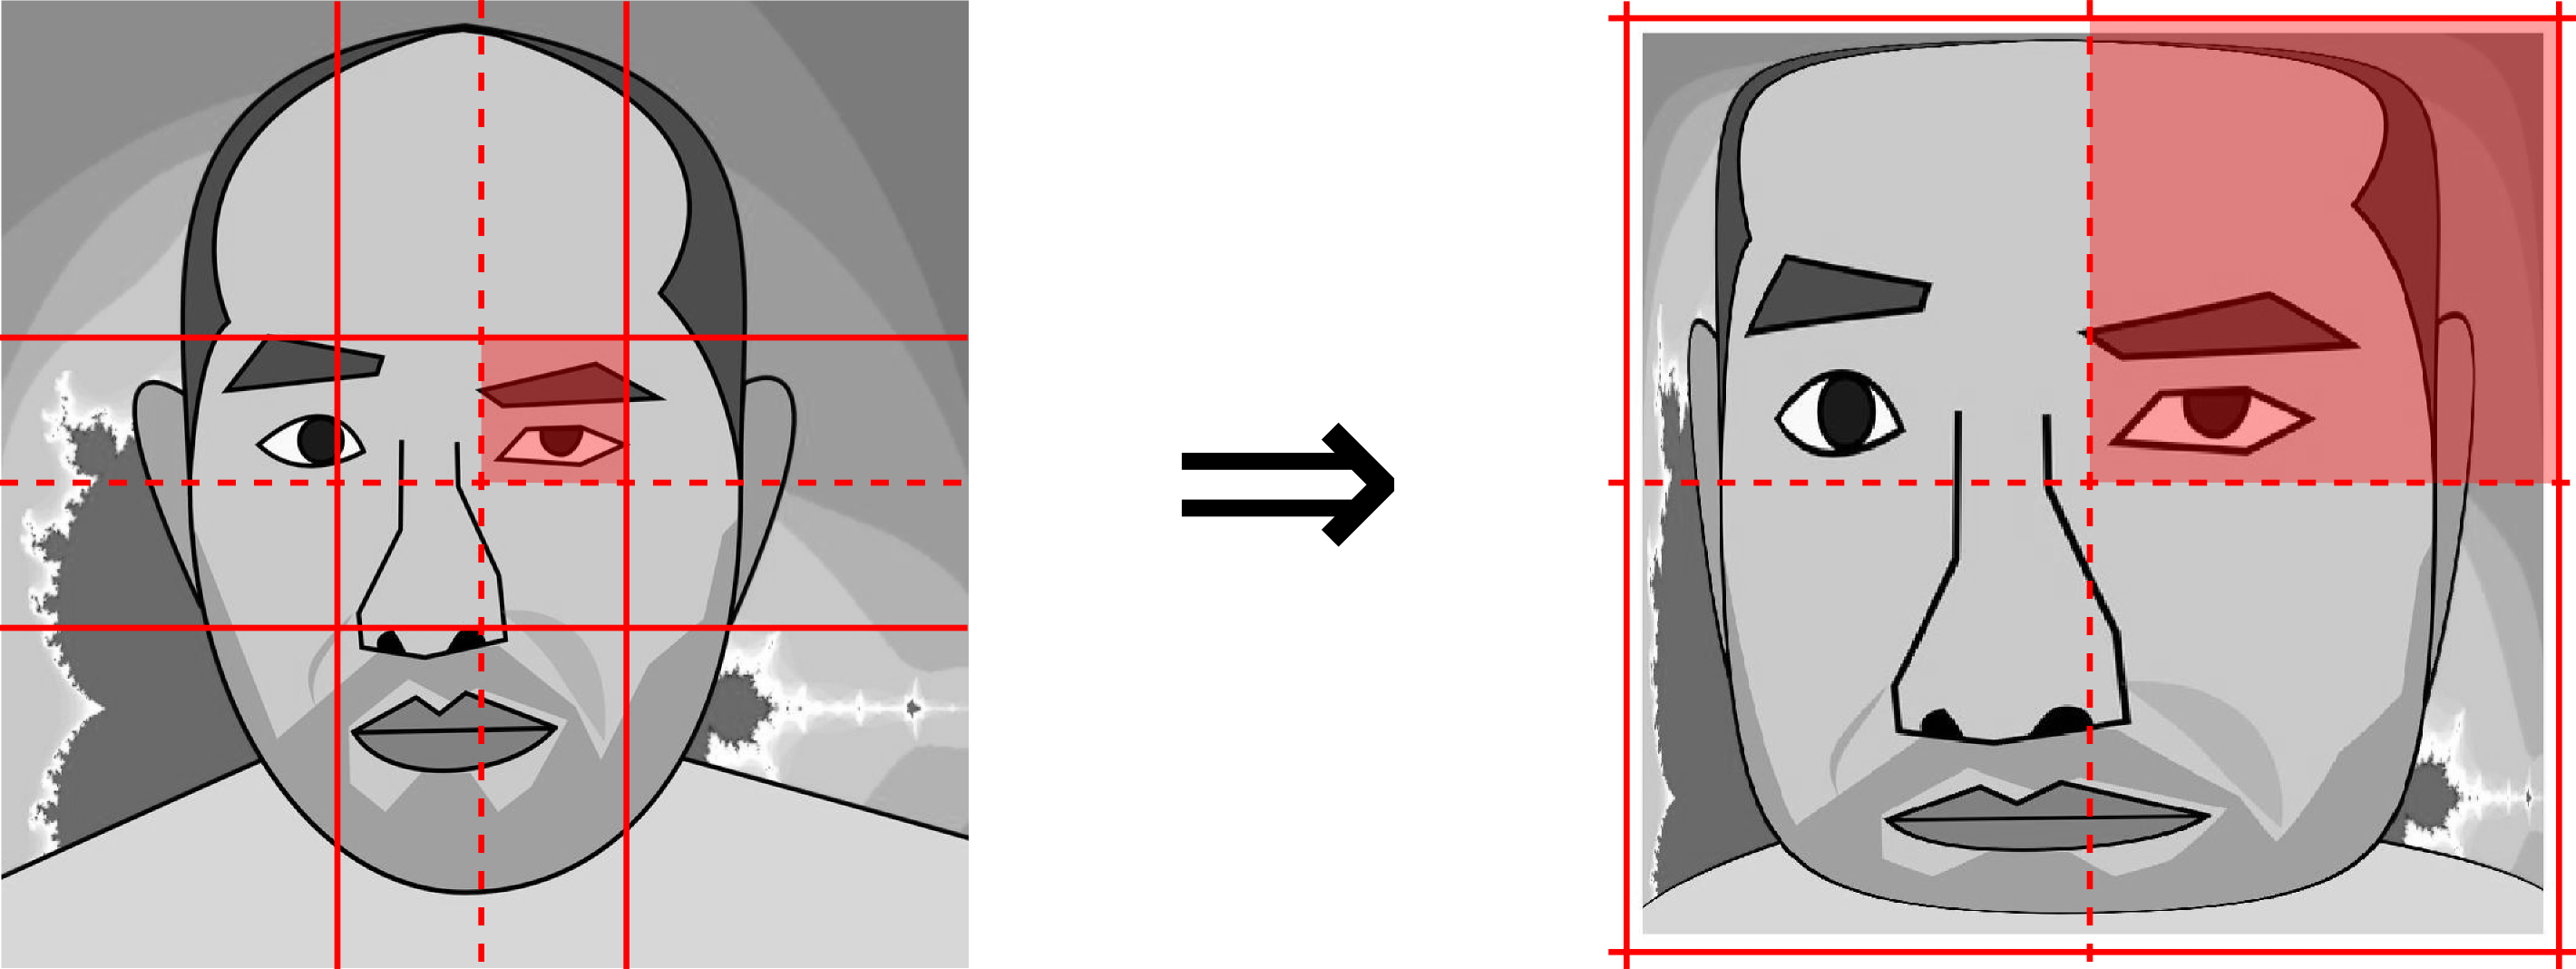
\includegraphics[scale=0.6]{sigmoid-transform-1.png}}}
\end{equation}

以下是\emp{一层}神经网络的变换,分解成 $W$ 和 $\sigmoid$ 两部分:
\begin{equation}
\vcenter{\hbox{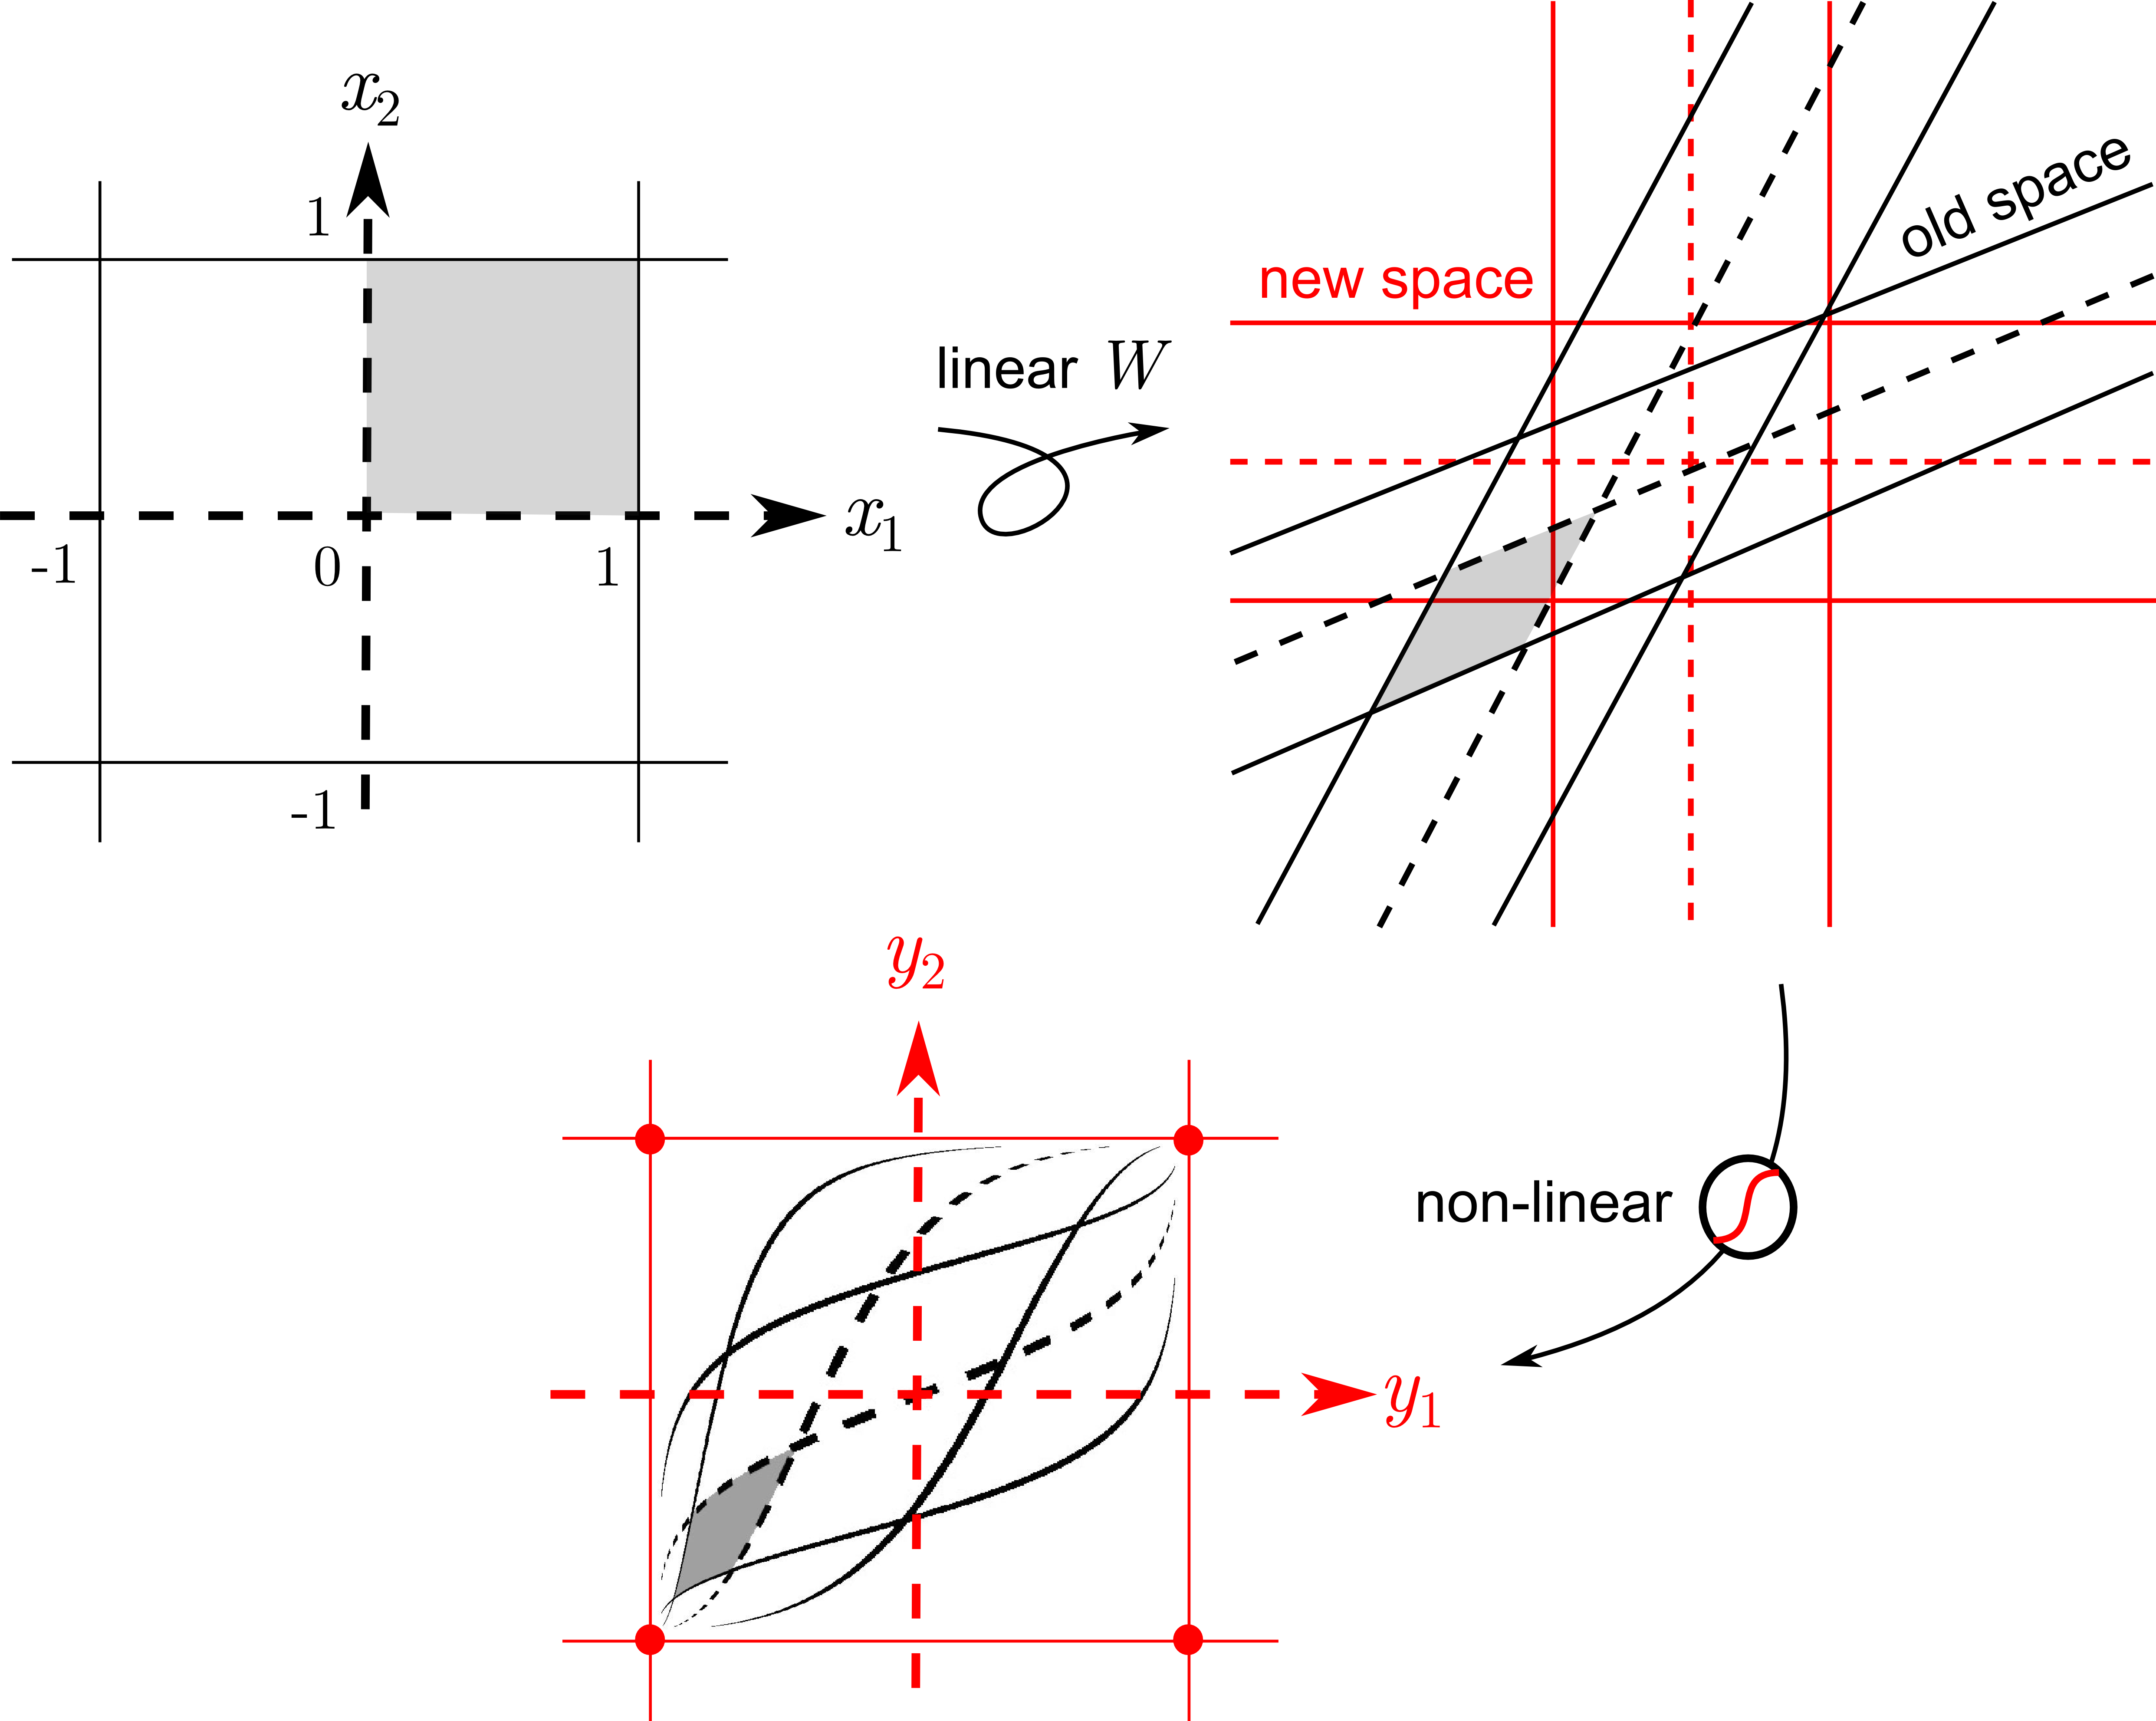
\includegraphics[scale=0.6]{NN-1-layer.png}}}
\end{equation}

\begin{tcolorbox}[colback=lightyellow, breakable, enhanced]
\section*{Sigmoid distortion 程式}

这个 Python 程式没有用到图像处理的 sampling 技巧,纯粹是简单的示範。 改编自 Prateek Joshi 的《OpenCV with Python by example》的 image warping 例子: \\  % 需要 install OpenCV 2 和 NumPy。
\footnotesize \url{https://www.packtpub.com/mapt/book/application_development/9781785283932}

\footnotesize
\begin{verbatim}
import cv2
import numpy as np
import math

img = cv2.imread("input.jpg", cv2.IMREAD_GRAYSCALE)
Y, X = img.shape                     # size of the image
print "X = ", X
print "Y = ", Y

img_out = np.zeros(img.shape, dtype=img.dtype)

k = 80.0                             # scaling factor (smaller = more distorted)

for y in range(Y):
    outsideX = False                 # out-of-boundary
    y0 = Y / (y + 0.5)               # y-position in original image scaled to [0,1]
    y1 = -k * math.log(y0 - 1.0)     # new position
    y2 = int(y1 + Y/2.0)             # adjust for mid-point
    if y2 >= Y or y2 < 0:            # out of boundary?
        outsideX = True
    for x in range(X):
        outsideY = False
        x0 = X / (x + 0.5)
        x1 = -k * math.log(x0 - 1.0)
        x2 = int(x1 + X/2.0)
        if x2 >= X or x2 < 0:
            outsideY = True
        if not (outsideX or outsideY):
            img_out[y,x] = img[y2,x2]
        else:
            img_out[y,x] = 255       # white color if out-of-bounds

cv2.imshow("Input", img)
cv2.imshow("Distorted", img_out)
cv2.imwrite("output.jpg", img_out)
\end{verbatim}
\normalsize

有兴趣的读者可以写一个游戏,「手动」地旋转 $W$ 矩阵,在 3D 或 4D 投影中分辨一些 patterns。
\end{tcolorbox}

%为简化讨论,现在只考虑 2 粒神经元的\emp{输入}和\emp{输出}空间(都是 2 度空间的平面):
%\begin{equation}
%\vcenter{\hbox{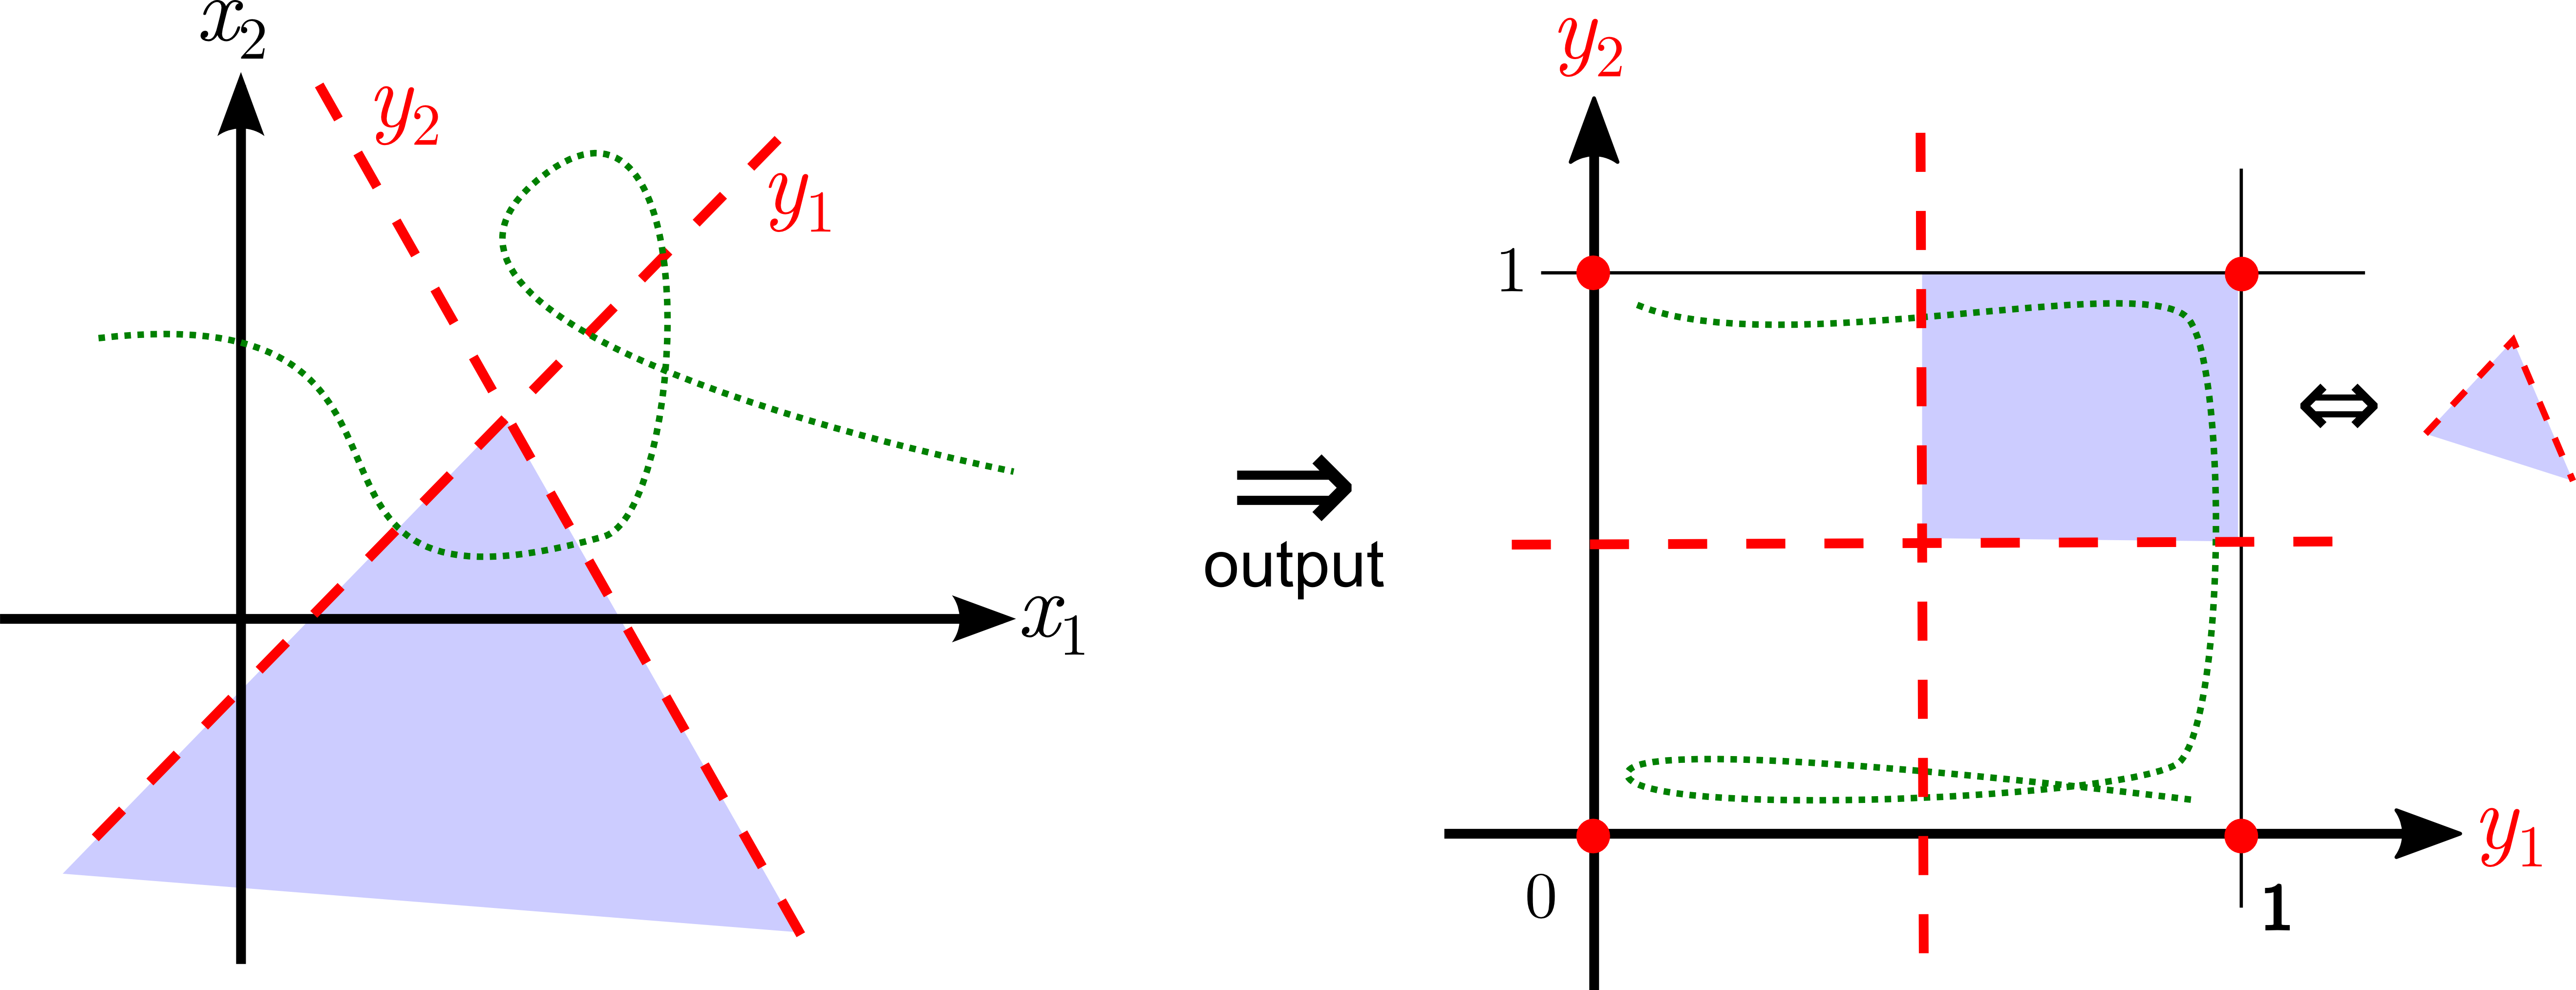
\includegraphics[scale=0.6]{linear-inequalities-3.png}}}
%\end{equation}
%因为 $\sigmoid$ 的缘故,输出的位置会趋近 hyper-cube 的那些 \emp{顶点} ({\color{red}{\textbullet}})。 这些顶点对应於输入空间中被割开的 regions。 例如 {\color{cerulean}{蓝色}}那块 region 对应於:
%\begin{equation}
%(y_1 = \mbox{yes}, y_2 = \mbox{yes}) \quad \Rightarrow \quad (1,1)
%\end{equation}
%当输入位置随{\color{darkgreen}{绿色}}线游荡时,输出会在 hyper-cube 的顶点之间跳来跳去。 妳可能觉得这样移动很无聊(因为顶点个数不多),但当神经元的个数 $n$ 增加时,hyper-cube 的顶点个数会以 $2^n$ 的速度增长。 

\section*{一层神经网络的 inverse}

现在再考虑,经过一层之后,如果在 target space 有一条 \emp{直线}(或者叫 linear discriminant),那么这条直线在 original space 会是什么形状?  这个形状就是 \emp{decision boundary},亦即是说,我们在 target 空间切了「线性的一刀」,在原空间这刀割的形状是怎样? 

在 target 空间的线性分割是:
\begin{equation}
a x' + b y' + c = 0
\end{equation}
神经网络的变换是:
\begin{equation}
(x' \; y') = \sigmoid W \genfrac(){0pt}{0}{x}{y}
\end{equation}
假设 $W = \mbox{id}$(忽略 $W$ 的作用),则变换简化成:
\begin{equation}
\begin{cases}
x' = \sigmoid x \\
y' = \sigmoid y
\end{cases}
\end{equation}
原空间的方程就是:
\begin{equation}
\frac{a}{1 + e^{-x}} + \frac{b}{1 + e^{-y}} + c = 0
\end{equation}
这家族的曲线(亦即是「刀的形状」)其中有些是这样的:
\begin{equation}
\vcenter{\hbox{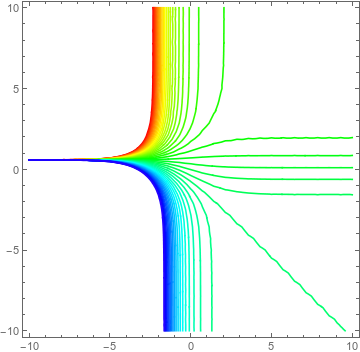
\includegraphics[scale=0.6]{curves2.png}}}
\end{equation}
%\includemedia[
%  activate=onclick,
%  width=0.5\textwidth
%]{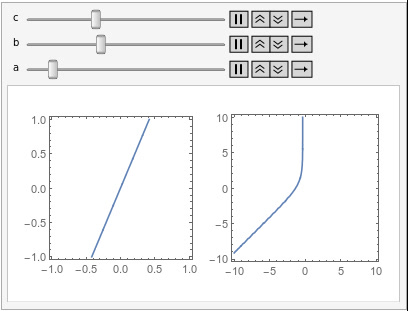
\includegraphics[scale=1.0]{movie.png}}{movie.flv}
换句话说: 在 target 空间中的直线切割,在原空间中被「压向中心」,变成有一个弯位的曲线,这是 $\sigmoid^{-1}$ 的作用。

\begin{tcolorbox}[colback=lightyellow, breakable, enhanced]
\section*{Mathematica 程式}

\footnotesize
\begin{verbatim}
Manipulate[
    GraphicsGrid[{{
        ContourPlot[a x + b y + c == 0, {x, -10, 10}, {y, -10, 10} ],
        ContourPlot[a/(1 + Exp[- k x]) + b/(1 + Exp[- k y]) + c == 0,
            {x, -10, 10}, {y, -10, 10} ]
        }}],
    {{a, .1}, -10, 10, .01},
    {{b, -.2}, -10, 10, .01},
    {{c, 0}, -10, 10, .05},
    {{k, 1}, 0.5, 5}]
\end{verbatim}
\normalsize

读者可以在 Mathematica 试验这些曲线的形状: 左边是 target 空间的直线,右边是它在原空间的曲线:

\begin{equation}
\vcenter{\hbox{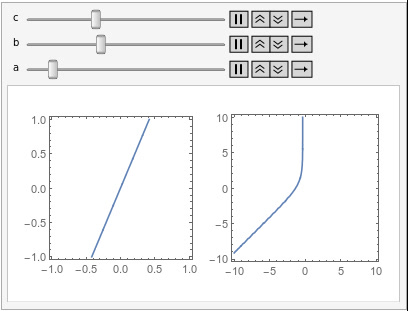
\includegraphics[scale=0.75]{Mathematica-manipulate.png}}}
\end{equation}
\end{tcolorbox}

注意,如果在 $\sigmoid$ 中加入参数 $\tau$ 变成:
\begin{equation}
\sigmoid (x) = \frac{1}{1 + e^{-\tau x}}
\label{tau-time}
\end{equation}
则当 $\tau \rightarrow \infty$ 时, $\sigmoid$ 变成 $\stepfunction$,而这些曲线也逐渐变成「角」的形状 \footnote{但其实当 $\tau \rightarrow \infty$ 时,在 target 空间只存在 4 个离散的顶点,所以那直线会变成 undefined。}:
\begin{equation}
\vcenter{\hbox{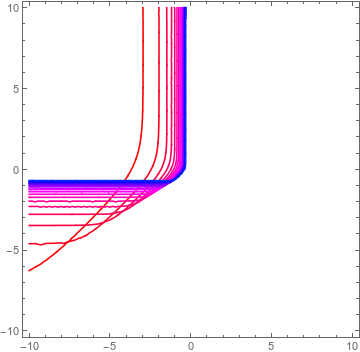
\includegraphics[scale=0.6]{towards-angular.png}}}
\end{equation}
这表示,在 $\tau \rightarrow \infty$ 时,decision boundary 会分割 4 个角位。 

讲了这么多,最重要的 insight 似乎是:  \uline{每个神经元所 represent 的其实只是一个 \emp{binary feature}}。 

% ***************** Does not work in XeLatex ***************
%\includemovie[
%	poster,
%	toolbar,
%	label=angular.u3d,
%	text=(angular.u3d),
%	3Daac=60.000000, 3Droll=0.000000, 3Dc2c=0.006653 -34.630001 0.000000, 3Droo=34.630001, 3Dcoo=0.006653 0.000000 0.000000,
%	3Dlights=CAD,
%]{\linewidth}{\linewidth}{angular.u3d}

\section*{多层神经网络}

多层只是单层的重复:
\begin{equation}
\boxed{output} \; \vect{y} = \sigmoid \stackrel{1}{W} \; \sigmoid \stackrel{2}{W} \; ..... \; \sigmoid \stackrel{L}{W} \; \vect{x}
\end{equation}
$L$ = total number of layers.

在我想像中,多层神经网络的运作好像「拉面条」: (这只是示意图)
\begin{equation}
\vcenter{\hbox{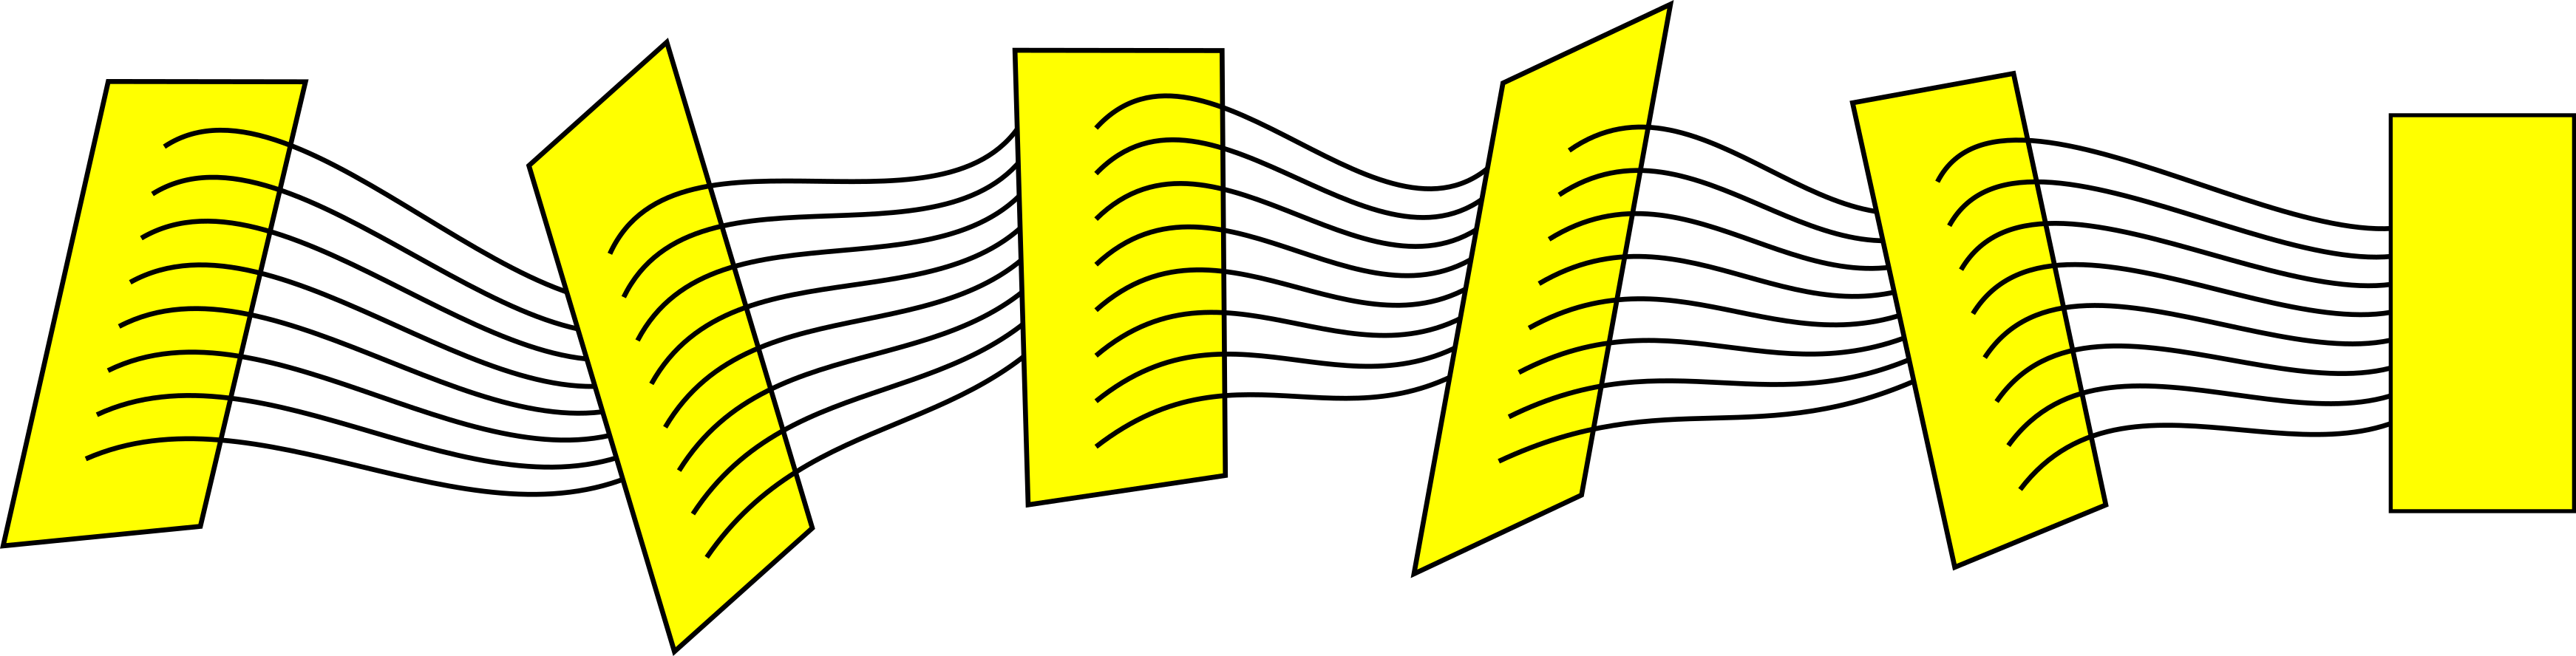
\includegraphics[scale=0.75]{ramen-noodle-1.png}}}
\end{equation}
如果在 (\ref{tau-time}) 式中的 $\tau \rightarrow 0$ \footnote{很奇怪地,当 $\tau \rightarrow 0$ 时,$\sigmoid (x) \rightarrow x$ 而不是 $1/2$,详细原因我也不知,反正 plot 出来是这样。},则这些「面条」会 ``unwind'' 成简单的一个线性变换:
\begin{equation}
\vcenter{\hbox{
\includegraphics[scale=0.75]{ramen-noodle-2.png}}}
\end{equation}
$\tau$ 可以看成是一个「另类时间」。 暂时我不知道这个想法有什么应用; 或许和 braid theory 有关?  但也可以看出: 每个神经元的数值输出,其实没有 fuzzy value 的意义,而仅仅是带有某些 topological 信息而已(亦即哪些点和哪些点邻近)。 

{\color{red}TO-DO}:  还有一件想做的事,是 plot 出多層神经網絡的 error surfaces。 记忆中好像看过这些 error surface 有「楼梯级」的形状,这可能解释为什么训练时 error 会有「骤然下降」的现象,而这可能不是 phase transition 现象,而纯粹是 error surface 固有的形状而已。 

\section*{和 Bayesian network 比较}

以上是对 NN 的「几何解释」,但其实有个更简单直接的解释是: NN 实现的是 \emp{命题逻辑} 的一种简单形式,例如以下的 Bayesian network 也可以看成是 NN 的一粒神经元,每个 node 代表一个命题: 
\begin{equation}
\vcenter{\hbox{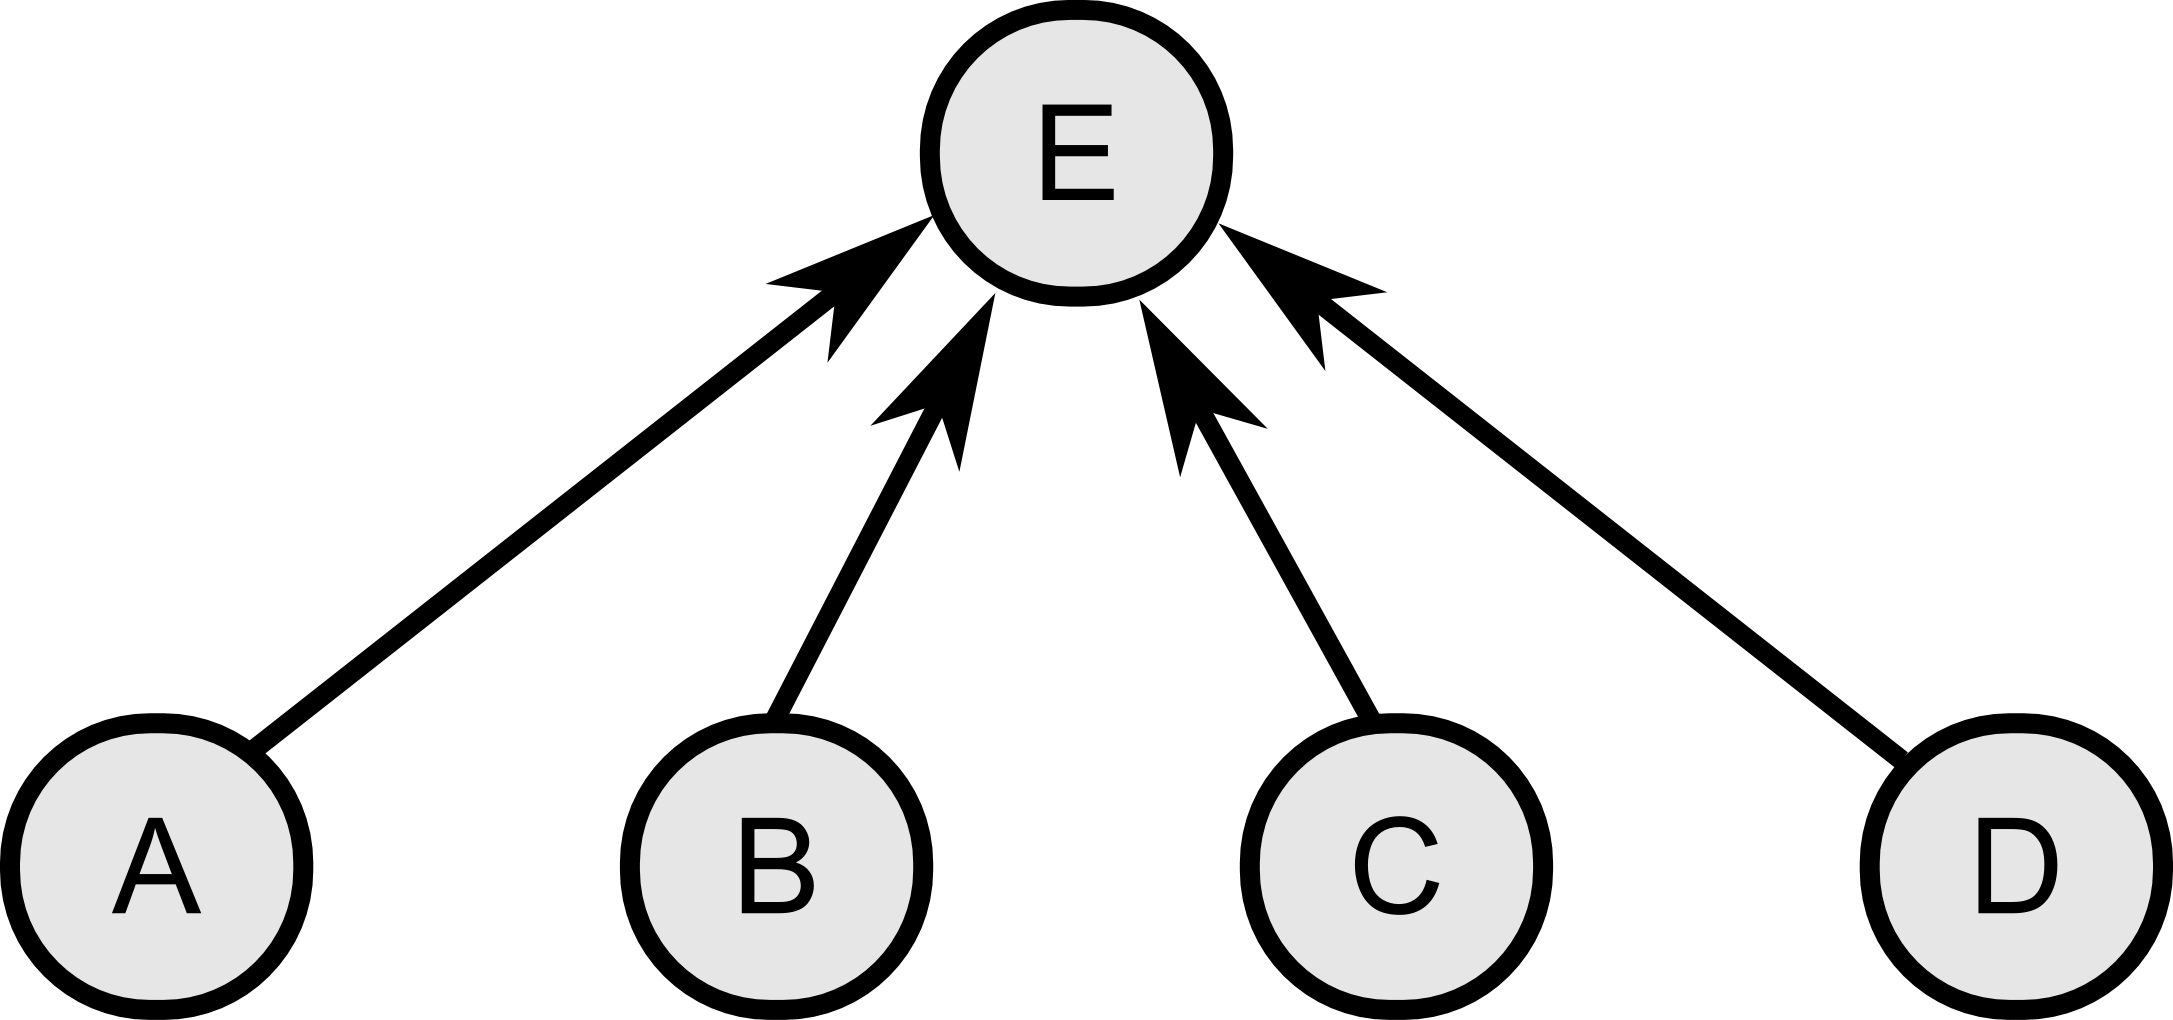
\includegraphics[scale=0.6]{flat-Bayes-net.png}}}
\end{equation}

但神经元的 $\sigmoid \sum$ 运算太简单,不足以计算概率的准确值。 举例来说,在 Bayesian network 中有 ``explaining away'' 的现象,例如以下的「遗书」如果存在,会令「自杀」的机率提升,但也令「他杀」的机率下降:
\begin{equation}
\vcenter{\hbox{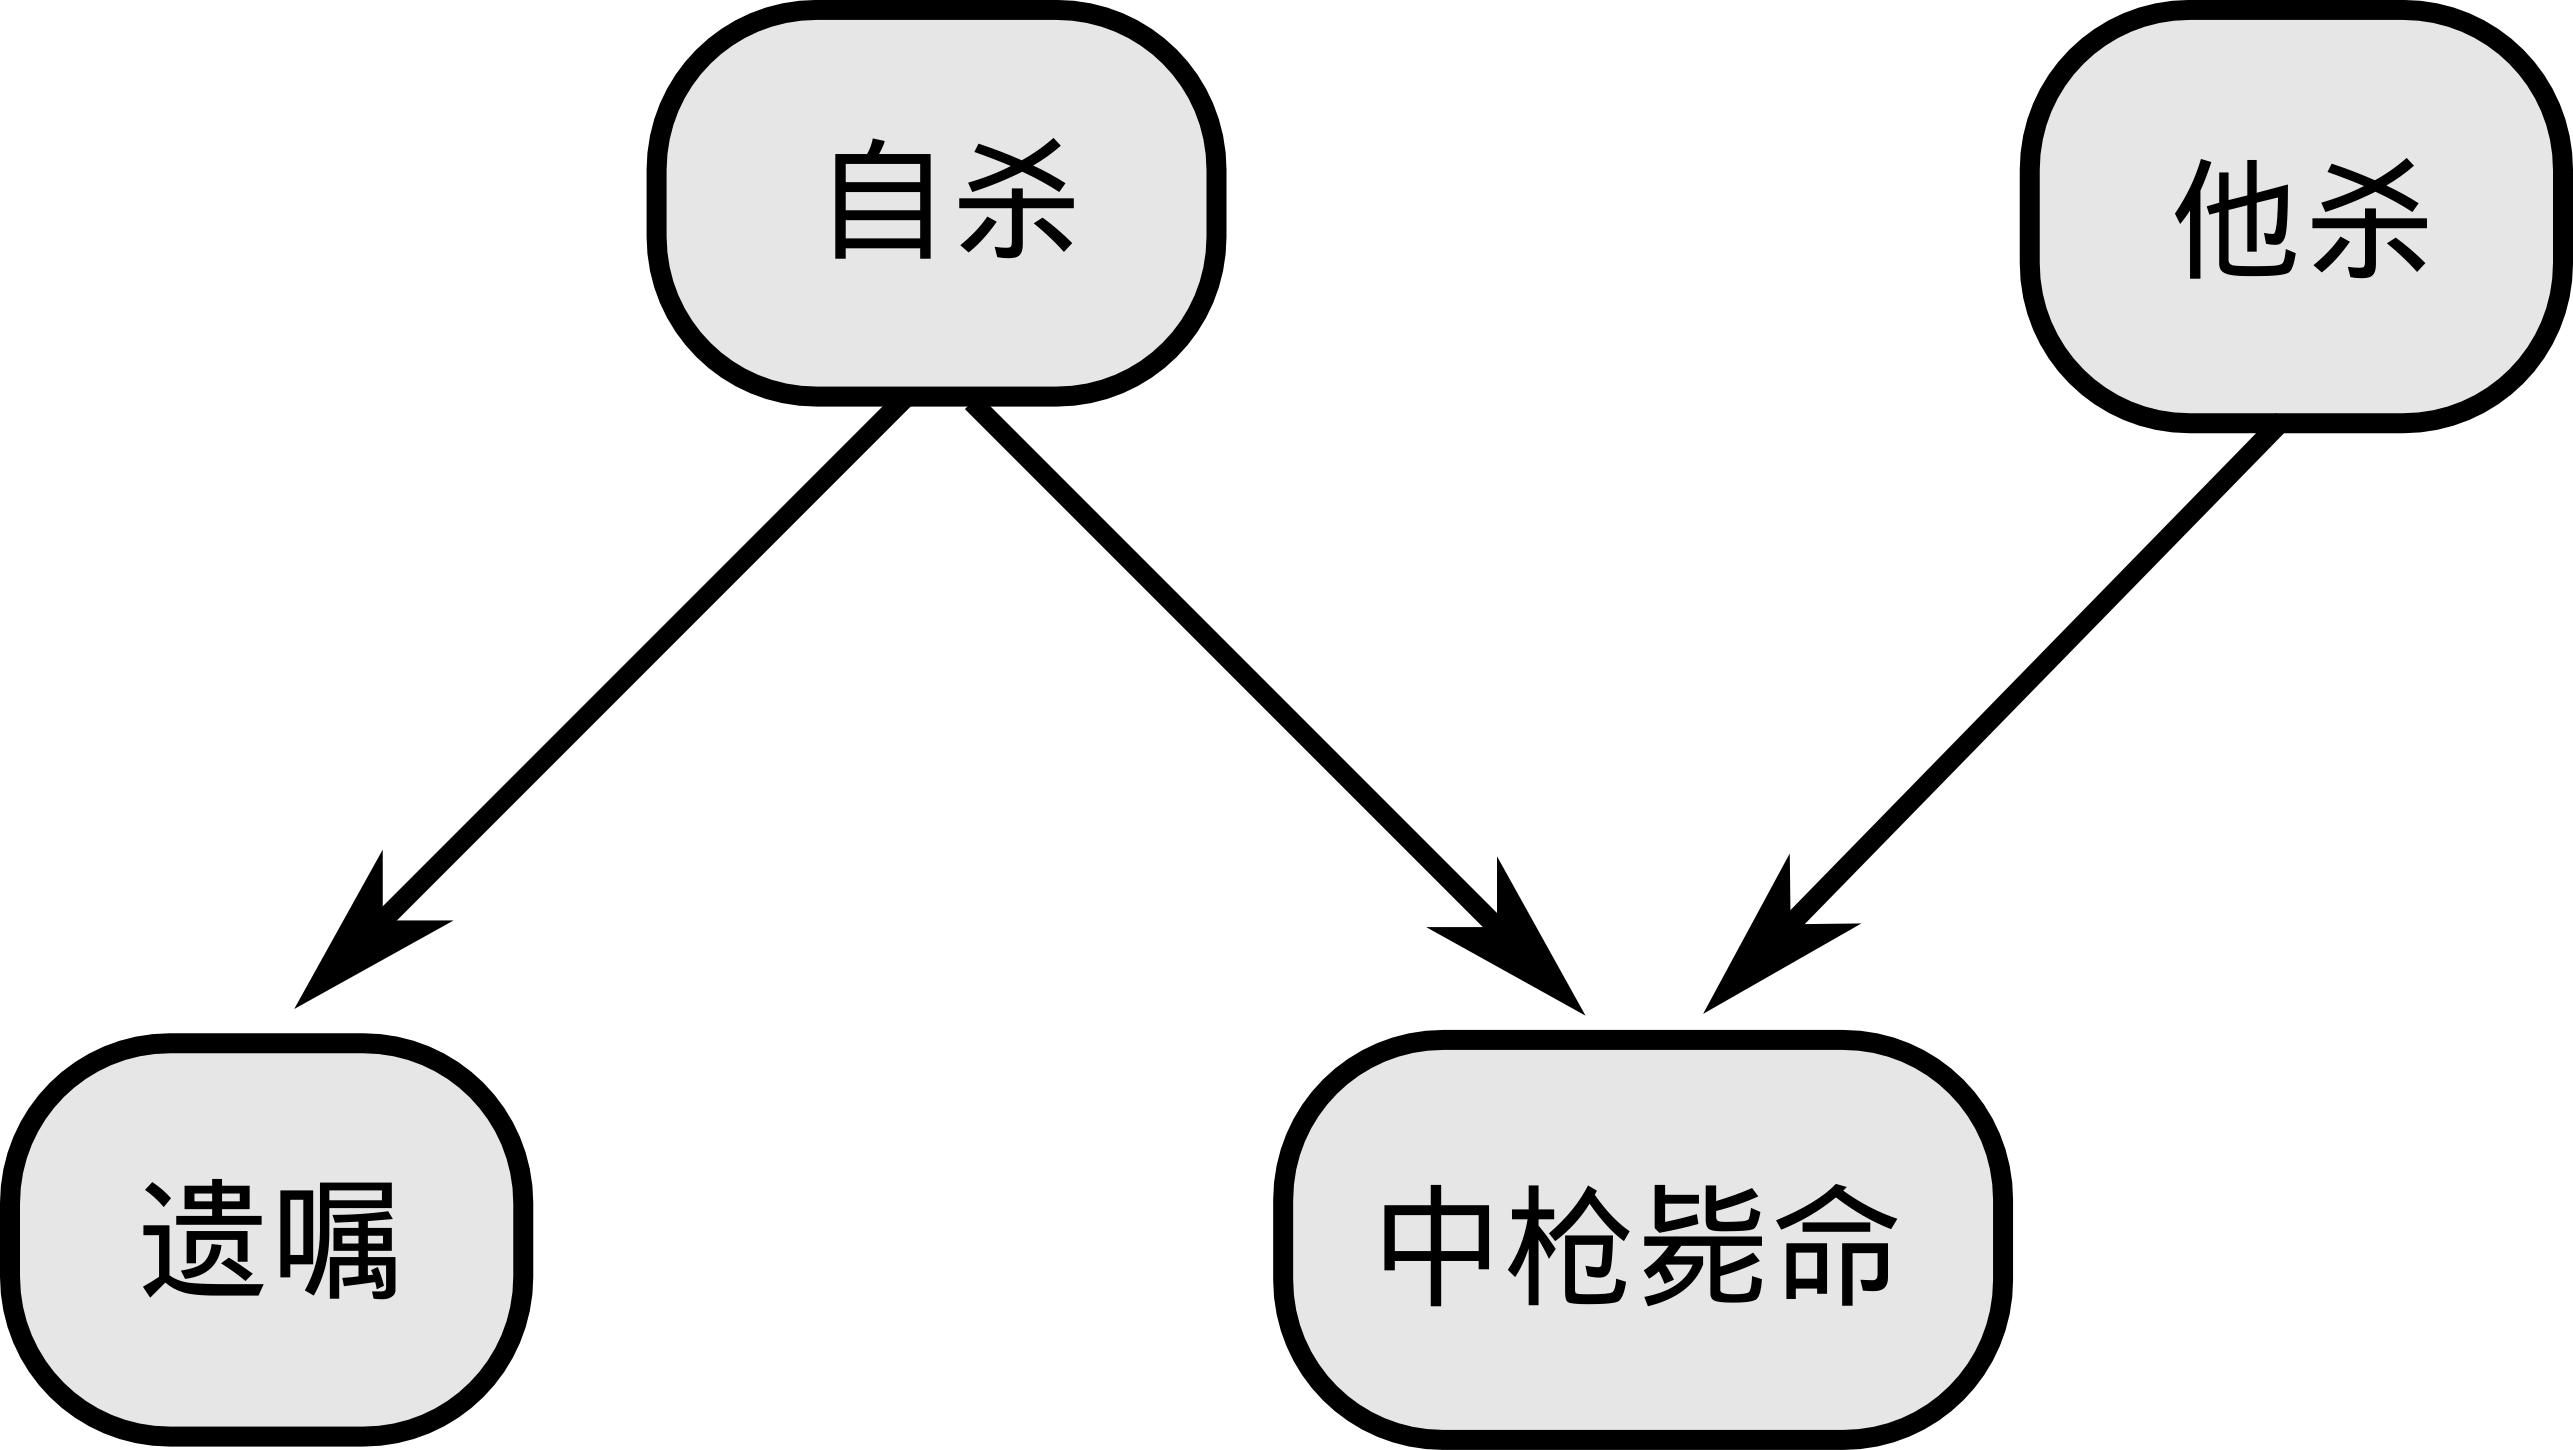
\includegraphics[scale=0.6]{suicide-note.png}}}
\end{equation}
换言之,在 Bayesian network 中概率的计算是有传递性的,它需要用到复杂的 \emp{belief propagation} 算法,这个算法复杂是因为它严格遵守概率论,但神经网络的简单性似乎难做到这效果。

% {\centering{\rule[0.5ex]{8cm}{1pt}}}

\section*{和 decision tree 比较}

% Decision tree 可不可以学习 features / representations?  有两种分析: 每个输入是一个 binary attribute; 或者每个 attribute 是一个 linear discriminant。  

重温一下 decision tree 的经典例子:
\begin{equation}
\vcenter{\hbox{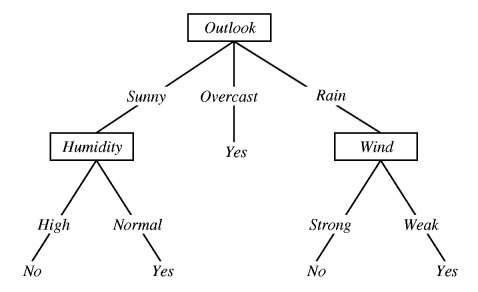
\includegraphics[scale=0.6]{decision-tree-classic-example.jpg}}}
\end{equation}
这是 training data:

\begin{equation}
\vcenter{\hbox{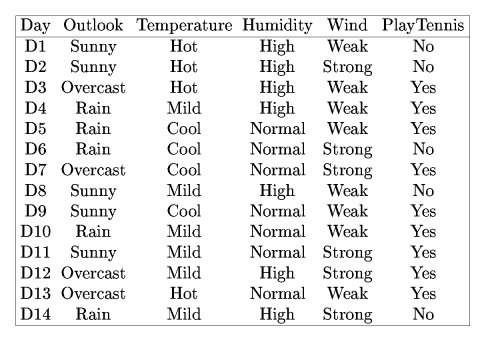
\includegraphics[scale=0.6]{decision-tree-classic-example-2.jpg}}}
\end{equation}
Decision tree 是根据 attribute-value pairs 来进行分类的。 为了较接近和神经网络比较,我假设这 decision tree 的每个 attribute 都是一个\emp{线性分割}:
\begin{equation}
\sum a_i x_i \stackrel{?}{>} 0
\end{equation}
Decision tree 有个特点: 每次分割之后,分开的两边是\emp{独立}处理的,彼此不再相关 \footnote{在图 (\ref{decision-tree-cuts}) 中分割很多次其实没有多大意义,因为输出只有 4 个「角位」而已。 有意义的分割在高维空间才看得出来。}:
\begin{equation}
\vcenter{\hbox{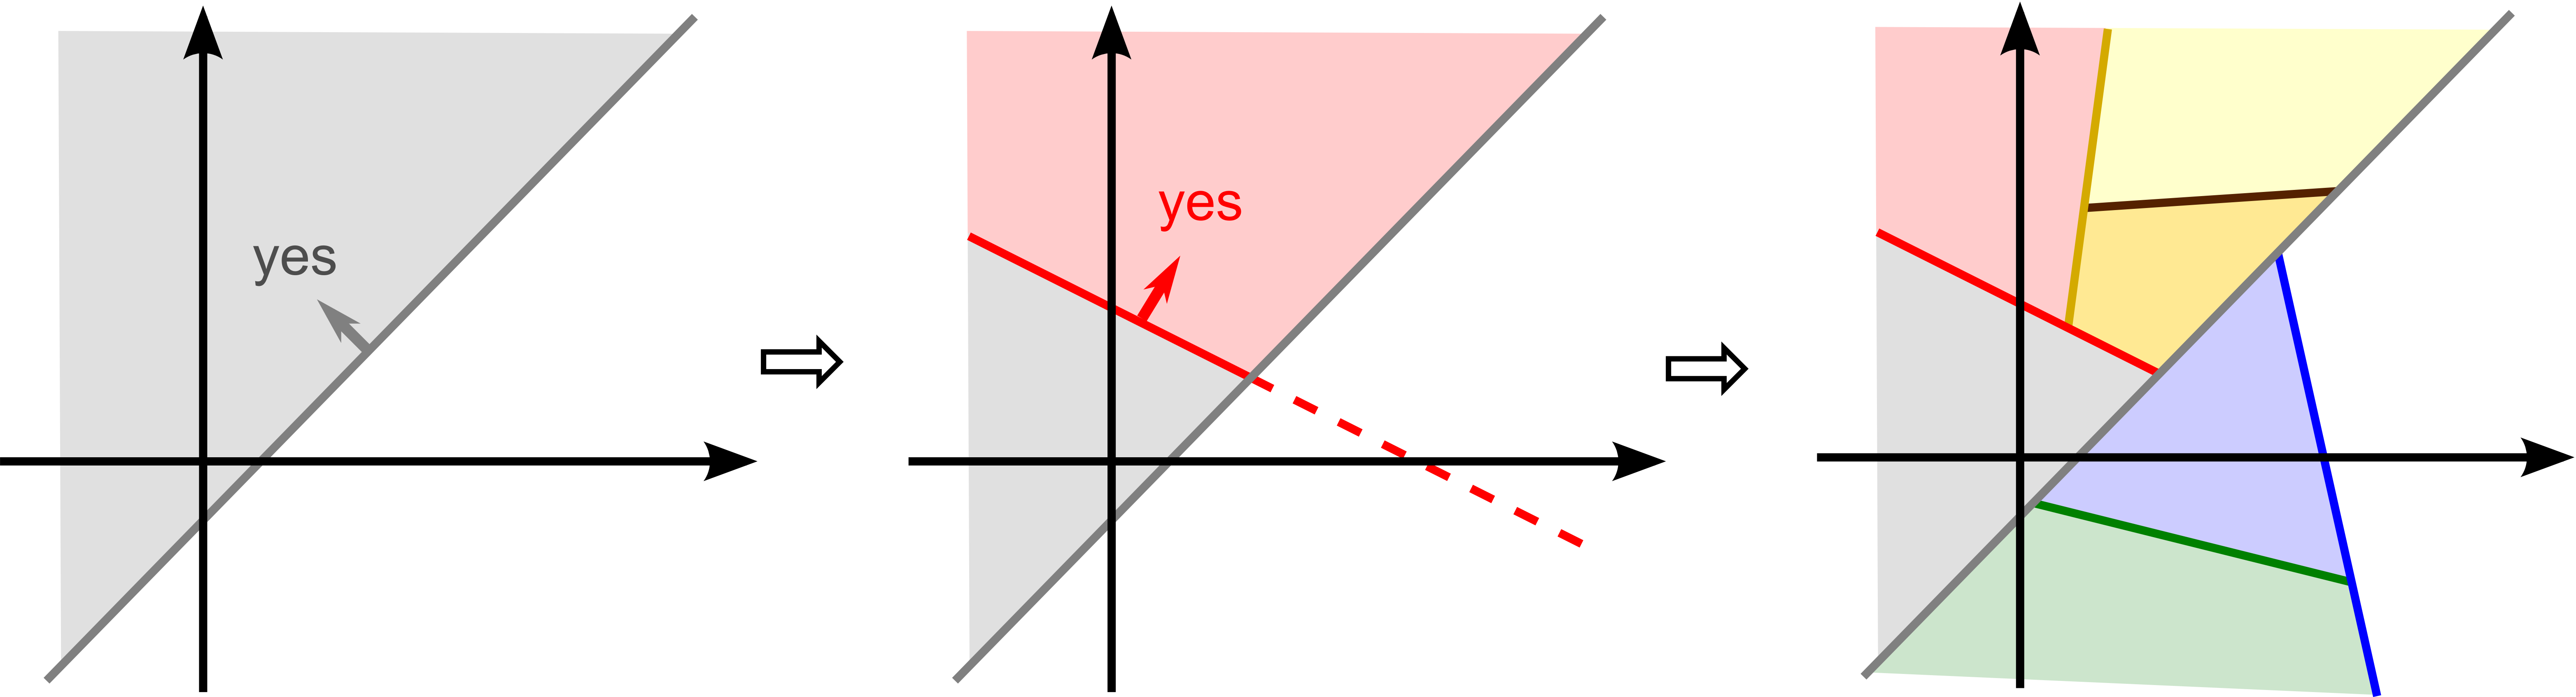
\includegraphics[scale=0.6]{decision-tree-cuts.png}}}
\label{decision-tree-cuts}
\end{equation}
例如在最上层做了~ 男生/女生~ 的分割后,接下来女生的分割可能是「漂亮」、「身材好」这些属性,而男生那边则是「高大」、「有钱」等; 男生和女生的重要属性不同。 可以说决策树做的是 ``\emp{shallow cut}'',和神经网络的 ``\emp{deep cut}'' 不同。 

观察多层 NN 的表达式:
\begin{equation}
\boxed{output} \; \vect{y} = \sigmoid \stackrel{1}{W} \; \sigmoid \stackrel{2}{W} \; ..... \; \sigmoid \stackrel{L}{W} \; \vect{x}
\end{equation}
可以看到,每一层的「分类」结果,\emp{全部}送到下一层再作分类。 这和 decision tree 的情况很不同: 后者在建立 \emp{分支} (branching) 之后,对每个分支的分类是独立的,即所谓 greedy algorithm。 这凸显出神经网络是一种很特殊的分类器,它自底层到高层、每层之间有「千丝万缕」的关系,所以能做到 representation learning 或 features learning 的效果。

\section*{和命题逻辑的关系}

早在 AI 初期,「AI 之父」 John McCarthy 已经意识到 NN 只是一种简单的命题逻辑,他觉得这是严重的局限。 但注意:如果 NN 底层的神经元是 sub-symbolic 的话,它可以有「创造」新命题的能力,这就比经典命题逻辑的表达力强很多了。 

\centering{ --- 完 --- }

% \href{http://genifer.googlecode.com/files/Genifer - induction (30 July 2012).pdf}{inductive learning (PDF, in English)}

%\bibliographystyle{plain} % or number or aaai ...
%\bibliography{AGI-book}

\end{document}
